\documentclass{article}
% \usepackage{xeCJK}
\usepackage{amsmath}
\usepackage{amssymb}
\usepackage{mathrsfs}
\usepackage{xcolor}
\usepackage{bm}
\usepackage{hyperref}
\usepackage{graphicx}
\usepackage{subcaption}
\usepackage{float}
\usepackage{multicol}
\usepackage[ruled,linesnumbered]{algorithm2e}

\bibliographystyle{plain}
\setlength{\parindent}{2em}
\usepackage{geometry}
\geometry{a4paper, left=2.54cm, right=2.54cm, top=3.18cm, bottom=3.18cm}

% 设置文章行距
% \renewcommand{\baselinestretch}{1.5}

% define reference format
\hypersetup{
    colorlinks=true,
    linkcolor=blue,
    urlcolor=blue,
    citecolor=blue,
    linkbordercolor=white
}

\title{\textbf{Chemotactic Chiral Active Matter}}
\author{Yichen Lu}

\begin{document}

\maketitle

\tableofcontents

\newpage
\section{Models}
\subsection{Definitions}
\subsubsection{Self-propelled dynamics}

\begin{subequations}
    \begin{align}
    \dot{x}_i&=v\cos \theta _i\;,
    \\
    \dot{y}_i&=v\sin \theta _i\;,
    \end{align}
    \label{eq:dotxy}
\end{subequations}

\subsubsection{Polar alignment dynamics}
\begin{itemize}
    \item Additive coupling: 
    \begin{equation}
        \label{eq:additionalCouplingDotTheta}
        \dot{\theta}_i=\omega _i+K\sum_{j=1}^{N}f\left( r_{ij} \right)\sin \left( \theta _j-\theta _i+\alpha \right)\;,
    \end{equation}
    \item Mean-field coupling by oscillator number:
    \begin{equation}
        \label{eq:swarmalatorDotTheta}
        \dot{\theta}_i=\omega _i+\frac{K}{N}\sum_{j=1}^N{f}\left( r_{ij} \right) \sin \left( \theta _j-\theta _i+\alpha \right) \;,
    \end{equation}
    which is similar to the swarmalator model.
    % \item Mean-field coupling by oscillator density:
    % \begin{equation}
    %     \dot{\theta}_i=\omega _i+\frac{KL^2}{\pi d_{0}^{2}N}\sum_{j=1}^N{f}\left( r_{ij} \right) \sin \left( \theta _j-\theta _i+\alpha \right) \;,
    % \end{equation}
    % where $d_0$ is the radius of the interaction circle.
\end{itemize}
Here,  $f\left( r_{ij} \right)$ is a function of $r=\left| \mathbf{r}_i-\mathbf{r}_j \right|$, and $K$ is the coupling strength. 
The function $f\left( r \right)$ can be defined as
\begin{enumerate}
    \item $f_H\left( r \right)=H\left( d_0-r \right),\;r_0>0$;
    \item $f_E\left( r \right)=e^{-\frac{r}{d_0}},\;r_0>0$.
\end{enumerate}
The natural frequencies $\omega_i$ are distributed with following two cases:
\begin{enumerate}
    \item \textbf{Single-chiral swarmalators:} The natural frequencies $\omega_i$ are distributed in $U\left( \omega _{\min},\omega _{\max} \right)$ for all swarmalators and $\omega _{\min}\omega _{\max}>0$.
    
    \item \textbf{Double-chiral swarmalators:} The frequencies are distributed in two symmetric uniform distributions, representing two types of chirality. Exactly half of the swarmalators have natural frequencies $\omega_i \sim U\left( \omega _{\min},\omega _{\max} \right)$ and the other half have natural frequencies $\omega_i \sim U\left( -\omega _{\max},-\omega _{\min} \right)$.
\end{enumerate}

\subsubsection{Chemotactic dynamics}

Consider two chemical fields $u\left( \mathbf{r},t \right), v\left( \mathbf{r},t \right)$ that are produced by the ensemble of two symmetrically chiral swarmalators. Swarmalators interact with the chemical field and move towards/against the regions with higher concentration, which can be described by the following equation ($i=1, 2, \dots, N$):
\begin{subequations}
    \begin{align}
        \dot{\mathbf{r}}_{i}^{s}&=v\mathbf{p}_{i}^{s}\\
        \dot{\theta}_{i}^{s}&=\omega _{i}^{s}+\alpha ^{s}\mathbf{p}_{i}^{s}\times \nabla u+\beta ^{s}\mathbf{p}_{i}^{s}\times \nabla v
    \end{align}
\end{subequations}
where $\alpha, \beta _{i}^{s}$ denote the ‘chemotactic’ coupling strength and $\mathbf{p}_i^{s}=(\cos \theta^{s} _i,\sin \theta _i^{s})$ is the unit vector pointing in the direction of the $i$-th swarmalator, $s\in\{p, n\}$ denotes the two chiral species. Here, we used the notation $\mathbf{a}\times\mathbf{b}=a_1 b_2-a_2 b_1$.

These two fields evolve as
\begin{subequations}
    \begin{align}
    \dot{u}&=k_0\sum_{j=1}^N{\delta \left( \mathbf{r}-\mathbf{r}_{j}^{p} \right)}-k_du+D_u\nabla ^2u\;,\\
    \dot{v}&=k_0\sum_{j=1}^N{\delta \left( \mathbf{r}-\mathbf{r}_{j}^{n} \right)}-k_dv+D_v\nabla ^2v\;,
    \end{align}
\end{subequations}
where $S_+$ and $S_-$ are the sets of two chiral swarmalators, $k_0$ is the production rate, $k_d$ is the decay rate, $D_{u,v}$ are the diffusion coefficients.

\subsubsection{Mixed phase dynamics}
\begin{subequations}
    \begin{align}
        \dot{\mathbf{r}}_i&=v\mathbf{p}_i\\
        \dot{\theta}_i&=\omega _i+\beta _{i}^{u}\mathbf{p}_i\times \nabla u+\beta _{i}^{v}\mathbf{p}_i\times \nabla v+\frac{K}{N}\sum_{j=1}^N{f}\left( \left| \mathbf{r}_j-\mathbf{r}_i \right| \right) \sin \left( \theta _j-\theta _i \right) \;,
    \end{align}
\end{subequations}

\subsubsection{Short format coarse graining}
We begin with Eq.~(\ref{eq:additionalCouplingDotTheta}), replacing the finite coupling distance alignment interaction with a pseudopotential (the '$\delta$'-interaction). This substitution is justified when the interaction is sufficiently short-ranged, making the specific shape of the associated interaction potential irrelevant to the dynamics of many swarmalators. The pseudopotential is defined as:
\begin{subequations}
    \begin{align}
        &\mathbf{\dot{r}}_{i}^{c}=v\mathbf{p}\left( \theta _{i}^{c} \right) \;,\\
        &\dot{\theta}_{i}^{c}=\omega _{i}^{c}+K\sum_{j=1}{\delta \left( \mathbf{r}_{j}^{c}-\mathbf{r}_{i}^{c} \right) \sin \left( \theta _{j}^{c}-\theta _{i}^{c} \right)}\notag\\
        &+K\sum_{j=1}{\delta \left( \mathbf{r}_{j}^{b}-\mathbf{r}_{i}^{b} \right) \left[ \sin \left( \theta _{j}^{b}-\theta _{i}^{b}+\alpha _0 \right) -\sin \alpha _0 \right]}\;,
    \end{align}
\end{subequations}
where $c\in\left\{+,-\right\}$ is the chirality of the swarmalator $i$ and $b=+$ if $c=-$ and vice versa.  
Then following \cite{DavidSDean_1996} we derive a continuum equation of motion for the combined $N$-swarmalator probability density
\begin{equation}
    \label{eq:globalContinuityDef}
    \rho ^c\left( \mathbf{r},\theta ,t \right) =\sum_{i=1}{\rho _{i}^{c}\left( \mathbf{r},\theta ,t \right)}\;,
\end{equation}
where $\rho _{i}^{c}\left( \mathbf{r},\theta ,t \right) =\delta \left( \mathbf{r}_{i}^{c}\left( t \right) -\mathbf{r} \right) \delta \left( \theta _{i}^{c}\left( t \right) -\theta \right)$ is the probability density of finding $i$-th swarmalator at position $\mathbf{r}$ with phase $\theta$ and chirality $c$ at time $t$.
Since the deterministic dynamical equation Eq.~ (\ref{eq:totalDynamics}) conserves the number of oscillators with a given natural frequency over time, the distribution function evolves according to a continuity equation of the following form:
\begin{equation}
    \frac{\partial \rho _{i}^{c}}{\partial t}=-\nabla \cdot \left( \rho _{i}^{c}v_{\mathbf{r}} \right) -\frac{\partial }{\partial \theta}\left( \rho _{i}^{c}v_{\theta}^{c,i} \right)\;.
    \label{eq:singleContinuity}
\end{equation}
Here, the velocity fields read
\begin{subequations}
    \begin{align}
        &v_{\mathbf{r}}\left( \mathbf{r},\theta ,t \right) =v\mathbf{p}\left( \theta \right) \;,\\
        &v_{\theta}^{c,i}\left( \mathbf{r},\theta ,t \right) =\omega _{i}^{c}+K\int{\text{d}\phi \rho^{c}\left( \mathbf{r},\phi ,t \right) \sin \left( \phi -\theta \right)}\notag\\
        &+K\int{\text{d}\phi \rho ^{b}\left( \mathbf{r},\phi ,t \right) \left[ \sin \left( \phi -\theta +\alpha _0 \right) -\sin \alpha _0 \right]}\;.
    \end{align}
\end{subequations}
Summing Eq.~(\ref{eq:singleContinuity}) over the $i$ and $c$ indices, and using the definition of the density $\rho ^c$ in Eq.~(\ref{eq:globalContinuityDef}), we obtain  
\begin{equation}
    \label{eq:globalContinuity}
    \begin{aligned}
        &\frac{\partial \rho ^c\left( \mathbf{r},\theta ,t \right)}{\partial t}=-v\mathbf{p}\left( \theta \right) \cdot \nabla \rho ^c\left( \mathbf{r},\theta ,t \right) -\frac{\partial}{\partial \theta}\Omega \left( \mathbf{r},\theta ,t \right)\\
        &+K\frac{\partial}{\partial \theta}\rho ^c\int{\text{d}\phi \rho ^c\left( \mathbf{r},\phi ,t \right) \sin \left( \phi -\theta \right)}\\
        &+K\frac{\partial}{\partial \theta}\rho ^c\int{\text{d}\phi \rho ^b\left( \mathbf{r},\phi ,t \right) \left[ \sin \left( \phi -\theta +\alpha _0 \right) -\sin \alpha _0 \right]}\;,
    \end{aligned}
\end{equation}
where $\Omega \left( \mathbf{r},\theta ,t \right) =\sum_{i=1}{\rho _{i}^{c}\left( \mathbf{r},\theta ,t \right) \omega _{i}^{c}}$.
Spatiotemporal dynamics of the ISS indicates $\forall i,c$, $\rho _{i}^{c}\left( \mathbf{r},\theta ,t \right) \equiv \rho _{\text{ISS}}\left( \mathbf{r},\theta ,t \right)$, which yields
\begin{equation}
    \Omega \left( \mathbf{r},\theta ,t \right) =\rho ^c\left( \mathbf{r},\theta ,t \right) \frac{\left( \omega _{\max}+\omega _{\min} \right)}{2}\;.
\end{equation} 

Transforming Eq.~(\ref{eq:globalContinuity}) to Fourier space, yields an equation of motion for the Fourier modes $\varrho _{k}^{c}\left( \mathbf{r},t \right) =\int{\rho ^c\left( \mathbf{r},\theta ,t \right) \text{e}^{\text{i}k\theta}\text{d}\theta}$ of $\rho^c$:
\begin{equation}
    \begin{aligned}
        \frac{\partial \varrho _{k}^{c}}{\partial t}&=-\frac{v}{2}\left[ \frac{\partial}{\partial x}\left( \varrho _{k+1}^{c}+\varrho _{k-1}^{c} \right) -\mathrm{i}\frac{\partial}{\partial y}\left( \varrho _{k+1}^{c}-\varrho _{k-1}^{c} \right) \right]\\
        &-\left[ \frac{\mathrm{i}k\left( \omega _{\max}+\omega _{\min} \right)}{2}\varrho _{k}^{c}-k^2 \right] \varrho _{k}^{c}\\
        &+\frac{\mathrm{i}Kk}{2\pi}\sum_{m=-\infty}^{\infty}{\varrho _{k-m}^{c}F_{-m}\varrho _{m}^{c}}\\
    \end{aligned}
\end{equation}

\subsubsection{Coarse graining}
We now follow the strategy in \cite{DavidSDean_1996} to consider the evolution of the density function for a single particle
\begin{equation}
    \rho _i\left( \mathbf{r},\theta ,\omega ,t \right) =\delta \left( \mathbf{r}_i\left( t \right) -\mathbf{r} \right) \delta \left( \theta _i\left( t \right) -\theta \right) g \left( \omega \right)\;, 
\end{equation}
which denotes the probability of finding a particle at position $\mathbf{r}$, with orientation $\theta$ and natural frequency $\omega$, where $g\left( \omega \right)$ is the time independent swarmalator frequency distribution. The density function $\rho _i$ satisfies the continuity equation, and we shall then demonstrate how one may write a closed equation for the global density
\begin{subequations}
    \begin{align}
        \rho \left( \mathbf{r},\theta ,\omega ,t \right) &=\sum_{i=1}^N{\rho _i\left( \mathbf{r},\theta ,\omega ,t \right)}\;,\\
        \varrho \left( \mathbf{r},\theta ,t \right) &=\int_{-\infty}^{+\infty}{\rho \left( \mathbf{r},\theta ,\omega ,t \right) \mathrm{d}\omega}\;.
        \label{eq:coarseDensitySub2}
    \end{align}
\end{subequations}
The derivation follows a well known argument. Consider an arbitrary function $f$ defined on the coordinate space of the system. Using the definition of the density it is a tautology
that
\begin{equation}
    \label{eq:arbitraryFunction}
    f\left( \mathbf{r}_i\left( t \right) ,\theta _i\left( t \right) ,\omega _i \right) =\iiint{\text{d}\mathbf{r}\text{d}\theta \text{d}\omega \rho _i\left( \mathbf{r},\theta ,\omega ,t \right) f\left( \mathbf{r},\theta ,\omega \right)}\;.
\end{equation}
Expanding the differential equation over the next time step $\delta t$ one obtains
\begin{equation}
    \begin{aligned}
        \frac{\text{d}f\left( \mathbf{r}_i,\theta _i,\omega _i \right)}{\text{d}t}&=\frac{\partial f\left( \mathbf{r}_i,\theta _i,\omega _i \right)}{\partial \mathbf{r}_i}\cdot \frac{\text{d}\mathbf{r}_i}{\text{d}t}+\frac{\partial f\left( \mathbf{r}_i,\theta _i,\omega _i \right)}{\partial \theta _i}\frac{\text{d}\theta _i}{\text{d}t}+\frac{\partial f\left( \mathbf{r}_i,\theta _i,\omega _i \right)}{\partial \omega _i}\frac{\partial \omega _i}{\partial t}\\
        &=\iiint{\text{d}\mathbf{r}\text{d}\theta \text{d}\omega \rho _i\left( \mathbf{r},\theta ,\omega ,t \right) \left( \frac{\partial f\left( \mathbf{r},\theta ,\omega \right)}{\partial \mathbf{r}}\cdot \frac{\text{d}\mathbf{r}}{\text{d}t}+\frac{\partial f\left( \mathbf{r},\theta ,\omega \right)}{\partial \theta}\frac{\text{d}\theta}{\text{d}t}+\frac{\partial f\left( \mathbf{r},\theta ,\omega \right)}{\partial \omega}\frac{\text{d}\omega}{\text{d}t} \right)}\\
        &=\iiint{\text{d}\mathbf{r}\text{d}\theta \text{d}\omega \left( \rho _i\left( \mathbf{r},\theta ,\omega ,t \right) \mathbf{\dot{r}}\cdot \nabla f\left( \mathbf{r},\theta ,\omega \right) +\rho _i\left( \mathbf{r},\theta ,\omega ,t \right) \dot{\theta}\frac{\partial}{\partial \theta}f\left( \mathbf{r},\theta ,\omega \right) \right)}\;.\\
    \end{aligned}
\end{equation}
Re-arranging the above integral by integration by parts we obtain
\begin{equation}
    \label{eq:arbitraryFunctionDt1}
    \frac{\text{d}f\left( \mathbf{r}_i,\theta _i,\omega _i \right)}{\text{d}t}=\iiint{\text{d}\mathbf{r}\text{d}\theta \text{d}\omega f\left( \mathbf{r},\theta ,\omega \right) \left( -\nabla \cdot \left( \rho _i\left( \mathbf{r},\theta ,\omega ,t \right) \mathbf{\dot{r}} \right) -\frac{\partial}{\partial \theta}\left( \rho _i\left( \mathbf{r},\theta ,\omega ,t \right) \dot{\theta} \right) \right)}\;.
\end{equation}
However, from \eqref{eq:arbitraryFunction} we may also deduce
\begin{equation}
    \label{eq:arbitraryFunctionDt2}
    \frac{\text{d}f\left( \mathbf{r}_i,\theta _i,\omega _i \right)}{\text{d}t}=\iiint{\text{d}\mathbf{r}\text{d}\theta \text{d}\omega f\left( \mathbf{r},\theta ,\omega \right) \frac{\partial \rho _i\left( \mathbf{r},\theta ,\omega ,t \right)}{\partial t}}\;.
\end{equation}
Comparing equations \eqref{eq:arbitraryFunctionDt1} and \eqref{eq:arbitraryFunctionDt2} we find (using the fact that $f$ is an arbitrary function) that
\begin{equation}
    \label{eq:continuityEquation}
    \frac{\partial \rho _i\left( \mathbf{r},\theta ,\omega ,t \right)}{\partial t}=-\nabla \cdot \left( \rho _i\left( \mathbf{r},\theta ,\omega ,t \right) \mathbf{\dot{r}} \right) -\frac{\partial}{\partial \theta}\left( \rho _i\left( \mathbf{r},\theta ,\omega ,t \right) \dot{\theta} \right)\;.
\end{equation}
We emphasize that this argument is standard and the only subtlety is that we have not carried out any thermal averaging at this point. Summing equation \eqref{eq:continuityEquation} over the $i$ and using the definition of the density $\rho$ we obtain
\begin{equation}
    \frac{\partial \rho \left( \mathbf{r},\theta ,\omega ,t \right)}{\partial t}=-\nabla \cdot \left( \rho \left( \mathbf{r},\theta ,\omega ,t \right) \mathbf{\dot{r}} \right) -\frac{\partial}{\partial \theta}\left( \rho \left( \mathbf{r},\theta ,\omega ,t \right) \dot{\theta} \right)\;.
\end{equation}
\begin{enumerate}
    \item[(1)] For the case of the phase coupling dynamics, the equation for the density $\rho$ is
    \begin{equation}
        \begin{aligned}
            \frac{\partial \rho \left( \mathbf{r},\theta ,\omega ,t \right)}{\partial t}&=-\nabla \cdot \left( \rho \left( \mathbf{r},\theta ,\omega ,t \right) v\mathbf{p}\left( \theta \right) \right) -\frac{\partial}{\partial \theta}\left( \rho \left( \mathbf{r},\theta ,\omega ,t \right) \left( \omega +G\sum_{j=1}^N{\sin \left( \theta _j-\theta \right) \delta \left( \mathbf{r}_j-\mathbf{r} \right)} \right) \right)\\
            &=-v\mathbf{p}\left( \theta \right) \cdot \nabla \rho \left( \mathbf{r},\theta ,\omega ,t \right) -\omega \frac{\partial}{\partial \theta}\rho \left( \mathbf{r},\theta ,\omega ,t \right) \\
            &-G\frac{\partial}{\partial \theta}\rho \left( \mathbf{r},\theta ,\omega ,t \right) \iiint{\text{d}\mathbf{r}'\text{d}\theta '\text{d}\omega '\rho \left( \mathbf{r}',\theta ',\omega ',t \right) \sin \left( \theta '-\theta \right) \delta \left( \mathbf{r}'-\mathbf{r} \right)}\;,
        \end{aligned}
    \end{equation}
    where $\mathbf{p}\left( \theta \right) =\left( \cos \theta ,\sin \theta \right)$. Then for the density $\varrho$ we have
    \begin{equation}
        \label{eq:coarseDensityAlign}
        \begin{aligned}
            \frac{\partial \varrho \left( \mathbf{r},\theta ,t \right)}{\partial t}&=-v\mathbf{p}\left( \theta \right) \cdot \nabla \varrho \left( \mathbf{r},\theta ,t \right) -\frac{\partial}{\partial \theta}\int_{-\infty}^{+\infty}{\omega \rho \left( \mathbf{r},\theta ,\omega ,t \right) \mathrm{d}\omega}\\
            &-G\frac{\partial}{\partial \theta}\varrho \left( \mathbf{r},\theta ,t \right) \iint{\mathrm{d}\mathbf{r}^{\prime}\mathrm{d}\theta^{\prime}\varrho \left( \mathbf{r}^{\prime},\theta^{\prime},t \right) \sin \left( \theta^{\prime}-\theta \right) \delta \left( \mathbf{r}^{\prime}-\mathbf{r} \right)}\\
        \end{aligned}
    \end{equation}
    \item[(2)] For the case of the chemotactic dynamics, the equation for the density $\rho^s$ is
    \begin{equation}
        \begin{aligned}
            \frac{\partial \rho ^s\left( \mathbf{r},\theta ,\omega ,t \right)}{\partial t}&=-\nabla \cdot \left( \rho ^s\left( \mathbf{r},\theta ,\omega ,t \right) v\mathbf{p}\left( \theta \right) \right) -\frac{\partial}{\partial \theta}\left( \rho ^s\left( \mathbf{r},\theta ,\omega ,t \right) \left( \omega +\alpha ^s\mathbf{p}\left( \theta \right) \times \nabla u+\beta ^s\mathbf{p}\left( \theta \right) \times \nabla v \right) \right)\\
            &=-v\mathbf{p}\left( \theta \right) \cdot \nabla \rho ^s\left( \mathbf{r},\theta ,\omega ,t \right) -\omega \frac{\partial}{\partial \theta}\rho ^s\left( \mathbf{r},\theta ,\omega ,t \right)\\
            &-\frac{\partial}{\partial \theta}\rho ^s\left( \mathbf{r},\theta ,\omega ,t \right) \alpha ^s\left[ \left| \nabla u \right|\sin \left( \theta +\varphi _u \right) +\left| \nabla v \right|\sin \left( \theta +\varphi _v \right) \right]
        \end{aligned}
    \end{equation}
    where $\varphi _c=\mathrm{arg}\left( -\partial _yc+\mathrm{i}\partial _xc \right) , c=u, v$. Then for the density $\varrho ^s$ we have
    \begin{equation}
        \label{eq:coarseDensityChemotactic}
        \begin{aligned}
            \frac{\partial \varrho ^s\left( \mathbf{r},\theta ,t \right)}{\partial t}&=-v\mathbf{p}\left( \theta \right) \cdot \nabla \varrho ^s\left( \mathbf{r},\theta ,t \right) -\frac{\partial}{\partial \theta}\int_{-\infty}^{+\infty}{\omega \rho ^s\left( \mathbf{r},\theta ,\omega ,t \right) \mathrm{d}\omega}\\
            &-\frac{\partial}{\partial \theta}\varrho ^s\left( \mathbf{r},\theta ,t \right) \alpha ^s\left[ \left| \nabla u \right|\sin \left( \theta +\varphi _u \right) +\left| \nabla v \right|\sin \left( \theta +\varphi _v \right) \right]\\
        \end{aligned}
    \end{equation}
\end{enumerate}
Next, let's determine the value of item
\begin{equation}
    \int_{-\infty}^{+\infty}{\omega \rho ^s\left( \mathbf{r},\theta ,\omega ,t \right) \text{d}\omega}\;.
\end{equation}
The uniform distribution of disorder state indicates $g\left( \omega \right) =\left[ 2\left( \omega _{\max}-\omega _{\min} \right) \right] ^{-1}$, which is an $\omega$-independent constant. Then we have
\begin{equation}
    \label{eq:omegaMulInt}
    \int_{-\infty}^{+\infty}{\omega \rho ^s\left( \mathbf{r},\theta ,\omega ,t \right) \text{d}\omega}=\begin{cases}
        \frac{1}{2}\rho ^s\left( \mathbf{r},\theta ,\omega ,t \right) \left( \omega _{\max}^{2}-\omega _{\min}^{2} \right) ,&		\text{Single} \text{Chirality}\\
        0,&		\text{Double} \text{Chirality}\\
    \end{cases}\;.
\end{equation}
Similarly, equation \eqref{eq:coarseDensitySub2} can be rewritten as
\begin{equation}
    \label{eq:coarseDensitySub2Rewrite}
    \varrho ^s\left( \mathbf{r},\theta ,t \right) =\rho ^s\left( \mathbf{r},\theta ,\omega ,t \right) \int_{-\infty}^{+\infty}{\text{d}\omega}=\begin{cases}
        2\left( \omega _{\max}-\omega _{\min} \right) \rho ^s\left( \mathbf{r},\theta ,\omega ,t \right) ,&		\text{Single} \text{Chirality}\\
        0,&		\text{Double} \text{Chirality}\\
    \end{cases}\;.
\end{equation}
Substituting equations \eqref{eq:coarseDensitySub2Rewrite} into \eqref{eq:omegaMulInt}, we obtain 

\subsubsection{Angular Fourier expansion of the phase-space distribution}
% The derivation of the evolution equation for the velocity field is actually much more complicated, and one has to resort to approximation schemes. 
As $\varrho(\mathbf{r},\theta,t)$ is a periodic function of $\theta$, it can be expanded in a Fourier series, defined as
\begin{equation}
    \hat{\varrho}_k(\mathbf{r},t)=\int_{-\pi}^\pi \varrho(\mathbf{r},\theta,t) \mathrm{e}^{\mathrm{i}k\theta}\mathrm{d}\theta\;.
\end{equation}
The inverse Fourier transform is
\begin{equation}
    \label{eq:inverseFourier}
    \varrho (\mathbf{r},\theta ,t)=\frac{1}{2\pi}\sum_{k=-\infty}^{\infty}{\hat{\varrho}_k(\mathbf{r},t)\mathrm{e}^{\mathrm{i}k\theta}\;.}
\end{equation}
In this framework, the uniform distribution $\varrho _0(\mathbf{r},\theta ,t)=\left( 2\pi \right) ^{-1}\varrho _{0}^{*}$ corresponds to $\hat{\varrho}_k(\mathbf{r},\omega,t)=\left( 2\pi \right) ^{-1}\varrho _{0}^{*}$ for $k=0$.

Let us use as a basis of the plane the two orthogonal vectors $\mathbf{p}_1=(1,0)$ and $\mathbf{p}_2=(0,1)$. In order to obtain an evolution equation for the velocity field, we multiply equations \eqref{eq:coarseDensityAlign} and \eqref{eq:coarseDensityChemotactic} by $\mathrm{e}\left(\theta\right)$ and integrate over $\theta$ from $-\pi$ to $\pi$. For equation \eqref{eq:coarseDensityChemotactic}, we obtain ($j=1,2$)
\begin{equation}
    \label{eq:angularFourierInt}
    \frac{\partial}{\partial t}\int_{-\pi}^{\pi}{\mathbf{e}_j\left( \theta \right) \varrho \left( \mathbf{r},\theta ,t \right) \mathrm{d}\theta}+v\sum_{l=1}^2{\frac{\partial}{\partial \mathbf{r}_l}\int_{-\pi}^{\pi}{\mathbf{e}_j\left( \theta \right) \mathbf{e}_l\left( \theta \right) \varrho \left( \mathbf{r},\theta ,t \right) \mathrm{d}\theta}}=\int_{-\pi}^{\pi}{\mathbf{e}_j\left( \theta \right) \left( I_{\mathrm{freq}}+I_{\mathrm{chem}} \right) \mathrm{d}\theta}\;,
\end{equation}
where 
\begin{subequations}
    \label{eq:angularFourierIntSub}
    \begin{align}
        &I_{\mathrm{freq}}=-\frac{\partial}{\partial \theta}\int_{-\infty}^{+\infty}{\omega \rho ^s\left( \mathbf{r},\theta ,\omega ,t \right) \mathrm{d}\omega}\;,\\
        &I_{\mathrm{chem}}=-\frac{\partial}{\partial \theta}\varrho ^s\left( \mathbf{r},\theta ,t \right) \alpha ^s\left[ \left| \nabla u \right|\sin \left( \theta +\varphi _u \right) +\left| \nabla v \right|\sin \left( \theta +\varphi _v \right) \right]\;.
    \end{align}
\end{subequations}
To proceed further, it is convenient to identify complex numbers with two-dimensional vectors, in such a way that $\mathbf{e}(\theta)$ is mapped onto $\mathrm{e}^{\mathrm{i}\theta}$. Then, in the same way, $v\hat{\varrho}_1\left( \mathbf{r},t \right) $ is associated with the momentum field $\mathbf{w}\left( \mathbf{r},t \right) =\rho \left( \mathbf{r},t \right) \mathbf{u}\left( \mathbf{r},t \right) $. Hence, we wish to rewrite equation \eqref{eq:angularFourierInt} in such complex notations. For later use, we shall write it in a slightly more general form, replacing $\mathrm{e}^{\mathrm{i}\theta}$ by $\mathrm{e}^{\mathrm{i}k \theta}$:
\begin{equation}
    \label{eq:angularFourierIntComplex}
    \frac{\partial}{\partial t}\int_{-\pi}^{\pi}{\mathrm{e}^{\mathrm{i}k\theta}\varrho \left( \mathbf{r},\theta ,t \right) \mathrm{d}\theta}+v\sum_{l=1}^2{\frac{\partial}{\partial \mathbf{r}_l}\int_{-\pi}^{\pi}{\mathrm{e}^{\mathrm{i}k\theta}\mathbf{e}_l\left( \theta \right) \varrho \left( \mathbf{r},\theta ,t \right) \mathrm{d}\theta}}=\int_{-\pi}^{\pi}{\mathrm{e}^{\mathrm{i}k\theta}\left( I_{\mathrm{freq}}+I_{\mathrm{chem}} \right) \mathrm{d}\theta}\;.
\end{equation}
Equation \eqref{eq:angularFourierInt} is recovered for $k = 1$, up to the mapping between complex numbers and two-dimensional vectors. The first term on the left-hand side is simply $\partial \hat{\varrho}_k/\partial t$. The second term on the left-hand side can be evaluated as follows: For $l=1,2$ and $k$ integer, let us define the complex quantity $Q_{l}^{\left( k \right)}\left( \mathbf{r},t \right)$ as 
\begin{equation}
    Q_l^{(k)}(\mathbf{r},t)=\int_{-\pi}^\pi\mathrm{d}\theta \mathrm{e}^{\mathrm{i}k\theta}\mathrm{e}_l(\theta)f(\mathbf{r},\theta,t).
\end{equation}
The following relations are then easily obtained:
\begin{equation}
    \begin{aligned}
        Q_{1}^{(k)}(\mathbf{r},t)&=\frac{1}{2}[\hat{f}_{k+1}(\mathbf{r},t)+\hat{f}_{k-1}(\mathbf{r},t)],\\
        Q_{2}^{(k)}(\mathbf{r},t)&=\frac{1}{2\mathrm{i}}[\hat{f}_{k+1}(\mathbf{r},t)-\hat{f}_{k-1}(\mathbf{r},t)].
    \end{aligned}
\end{equation}


The right-hand side of equation \eqref{eq:angularFourierIntComplex} is computed by inserting the Fourier series expansion \eqref{eq:inverseFourier} into equations \eqref{eq:angularFourierIntSub}. 
After a rather straightforward calculation, one finds

% \begin{equation}
%     Q_1^{(k)}(\mathbf{r},t)=\frac{1}{2}[\hat{f}_{k+1}(\mathbf{r},t)+\hat{f}_{k-1}(\mathbf{r},t)],\\Q_2^{(k)}(\mathbf{r},t)=\frac{1}{2\mathrm{i}}[\hat{f}_{k+1}(\mathbf{r},t)-\hat{f}_{k-1}(\mathbf{r},t)].
% \end{equation}


\subsubsection{Order Parameters}
Some order parameters can be introduced to measure the level of spatiotemporal coordinations among swarmalators and distinguish the different collective states of the system. Firstly, the usual order parameter to measure the global phase synchronization among swarmalators can be defined as the following complex function:
\begin{equation}
    Z\left( t \right) =R\left( t \right) \mathrm{e}^{\textrm{i}\psi(t)}=\frac{1}{N}\sum_{j=1}^N{\mathrm{e}^{\textrm{i}\theta _j(t)}}\;,
\end{equation}
where $\textrm{i}=\sqrt{-1}$. The degree modulus $R(t)=\left|Z(t)\right|$ is the absolute value of the mean of the complex numbers $e^{\textrm{i}\theta _i}$, which can be interpreted as the absolute value of the mean normalized velocity of all swarmalators. When $R\approx 1$, swarmalators are fully phase synchronized, and when $R\approx0$, swarmalators are phase incoherent.

The order parameter $R$ is not enough to measure the emergence of partial clustered phase synchronization of swarmalators. Therefore a local order parameter can be introduced to measure the clustered synchronization:
\begin{equation}
    Z_c^k (t) = R_c^k \left( t \right) \mathrm{e}^{\textrm{i}\psi_c^k (t)} =  \frac{1}{\left| C_k\left( t \right) \right|}\sum_{j\in C_k\left( t \right)}{\mathrm{e}^{\mathrm{i}\theta _j\left( t \right)}} \;,
\end{equation}
$N_c$ is the number of clusters, $C_k$ is the $k$-th cluster, and $\left| C_k \right|$ is the number of swarmalators in the $k$-th cluster (see the details of the determination of clusters in Appendix). An averaged global order parameter can be further introduced as
\begin{equation}
    R_c\left( t \right) =\frac{1}{N_c\left( t \right)}\sum_{k=1}^{N_c\left( t \right)}{R^k_c (t)}\;.
\end{equation}
As the swarmalators within the $k$-th cluster are fully synchronized, $R_c^k\approx 1$, and therefore also globally $R_c\approx 1$.

Except the study for phase coherence, other order parameters can be defined to further describe the locking of the frequencies of swarmalators under the chiral condition. One first introduce a cluster frequency difference to measure the chiral synchronizability of swarmalators within a cluster as
\begin{equation}
    \Delta \Omega_c^k = \frac{1}{\left| C_k \right|^2}\sum_{i,j\in C_k}{\left( \left< \dot{\theta}_i \right> -\left< \dot{\theta}_j \right> \right) ^2} ,
    \label{eq:clusterfrequency}
\end{equation}
where $\left< \dot{\theta}_i \right>$ is the average phase velocity of the $i$-th cluster, which can be defined by
\begin{equation}
    \left< \dot{\theta}_i \right> =\lim_{T\rightarrow \infty} \frac{1}{T}\int_{t_0}^{t_0+T}{\dot{\theta}_i\left( t \right) \mathrm{d}t}\;.
    \label{eq:frequency}
\end{equation}
Then a global frequency difference of clusters is
\begin{equation}
    \Delta \Omega_c =\frac{1}{N_c}\sum_{k=1}^{N_c} {\Delta \Omega_c^k}\;.
    \label{eq:globalcluster}
\end{equation}
% Yichen: 暂时没有用到这个\Delta\Omega,所以先注释掉
% Of course it is natural to introduce a global frequency difference without the identification of multiple clusters as
% \begin{equation}
%     \Delta \Omega =\frac{1}{N^2}\sum_{i,j=1}^{N}{\left( \left< \dot{\theta}_i \right> -\left< \dot{\theta}_j \right> \right) ^2 }\;.
%     \label{eq:frequencydifference}
% \end{equation}
For any cluster $k$, one can assume that $\left< \dot{\theta}_i \right>\in \left[a, b\right]$. Then the expectation of $\Delta \Omega_c^k$ can be calculated as
\begin{equation}
    E\left( \Delta \Omega _{c}^{k} \right) =2E\left( \left< \dot{\theta}_i \right> ^2 \right) -2E\left( \left< \dot{\theta}_i \right> \left< \dot{\theta}_j \right> \right)\;.
\end{equation}
For different cases of bounds, the value is
\begin{equation}
    E\left( \Delta \Omega _{c}^{k} \right) \begin{cases}
        =0,&		ab\geqslant 0\\
        >0,&		ab<0\\
    \end{cases}
\end{equation}
Therefore, if $n\rightarrow\infty$ and the average phase velocities of swarmalators within the cluster are all positive, all negative, $\Delta \Omega _{c}^{k}\approx0$, and we name this case as the \textit{chirality-locked cluster}. Otherwise, $\Delta \Omega _{c}^{k}>0$. 
When $\Delta\Omega_c \approx 0$, the swarmalators will organize to form several clusters, within each cluster swarmalators are chirality-locked. 
% When $\Delta\Omega \approx 0$, all swarmalators are frequency locked. 
Note that chirality locking is different from phase locking, as the chirality-locked swarmalators can have different phase velocities, which also means that they can have different rotational radii. 
Obviously, chirality locking is a more loose condition than phase locking. 

All the above order parameters measure different aspects of coordination in the phases of swarmalators. Because the phase variable describes the alignment of a swarmalator, various synchrony states imply the motion alignment of swarmalators in the swarming dynamics. 
% In the following discussions, we will further define more order parameters that are necessary to depict the spatial swarming ordering. 
In the following discussions, we further define an order parameter to depict the spatial swarming ordering:
\begin{equation}
    \label{eq:relativeNumber}
    N_r\left( t \right) =\frac{1}{N}\frac{1}{N_c\left( t \right)}\sum_{k=1}^{N_c\left( t \right)}{\left| C_k\left( t \right) \right|}\;.
\end{equation}
$N_r$ is the relative number of swarmalators in the clusters, which measures the spatial condensation of swarmalators. When $N_r\approx 1$, swarmalators are fully spatially condensed, and when $N_r\approx 0$, swarmalators are spatially dispersed. 

% \newpage
% \section{Results}
% \subsection{Signle-chiral Swarmalators}
% \begin{figure}[H]
%     \includegraphics[width=\textwidth]{./figs/MonoChiralPhaseDiagram.pdf}
%     \caption{
%         \label{fig:MonoPhaseDiagram} 
%         Phase diagram and snapshots of mono-chiral swarmalators.
%         \textbf{(a)} Phase diagram in the $(d_0$-$\lambda)$ plane. 
%         % The boundaries between states are analytical approximations given by Section~\ref{sec:phaseDiagrams}.
%         For the sake of clarity, the scale of $\lambda$ and $d_0$ is non-uniform.
%         \textbf{(b)}, The snapshots of CS ($\lambda=0.08,\ d_0=0.1$). 
%         \textbf{(c)}, DS ($\lambda=0.01,\ d_0=0.1$).
%         \textbf{(d)}, CLS ($\lambda=0.3,\ d_0=1$).
%         \textbf{(e)}, CLS ($\lambda=0.02,\ d_0=2$). The position and direction of each arrow are the instantaneous spatial position and phase of a swarmalator, respectively, and the color of the arrow denotes the corresponding natural frequency.
%     }
% \end{figure}

% \begin{figure}[H]
%     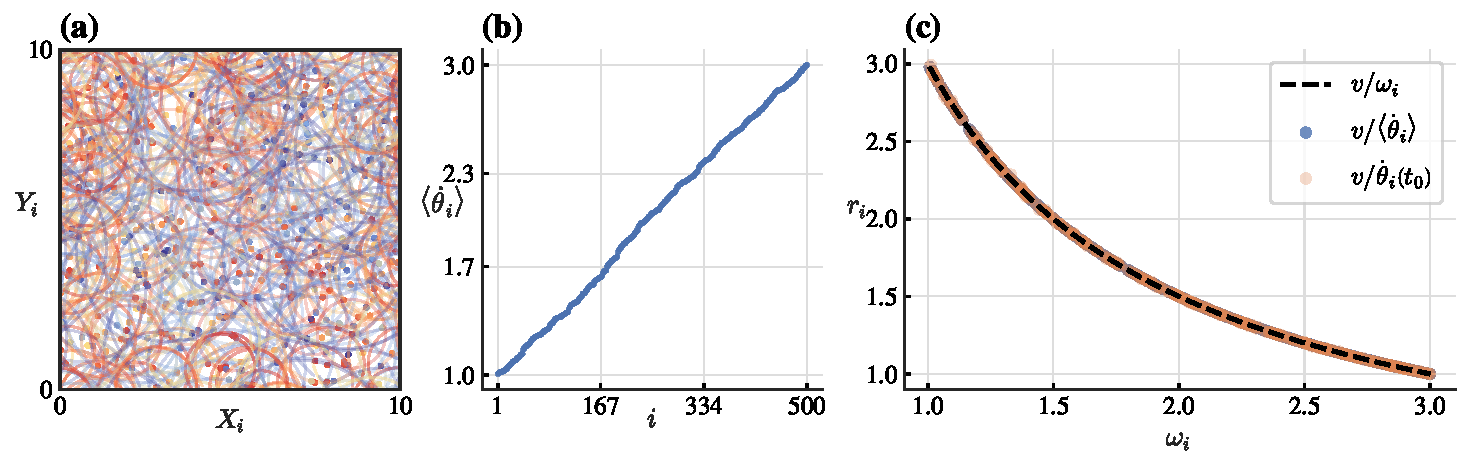
\includegraphics[width=\textwidth]{./figs/mono-DS.pdf}
%     \caption{
%         \label{fig:mono-DS} Swarming properties of DS for $\lambda =0.01$, $d_0 =0.1$. 
%         \textbf{(a)}: The orbits and the instantaneous rotation centers $\left\{ \mathbf{c}_i (t)\right\}$ of swarmalators. The color denotes the natural frequency.
%         \textbf{(b)}: The profile of the averaged frequencies $\langle \dot{\theta}_i \rangle$.
%         \textbf{(c)}: The instantaneous rotation radii $ r_i^{eff}$ and the average rotation radii $v/\langle \dot{\theta}_i \rangle$ against the natural frequencies $\omega_i$. The black dashed line is the relation $r_i^0 = v/\omega_i$ for the uncoupled case.
%     }
% \end{figure}

% \subsubsection{Spatial Clustering in Circling State}

% \begin{figure}[H]
%     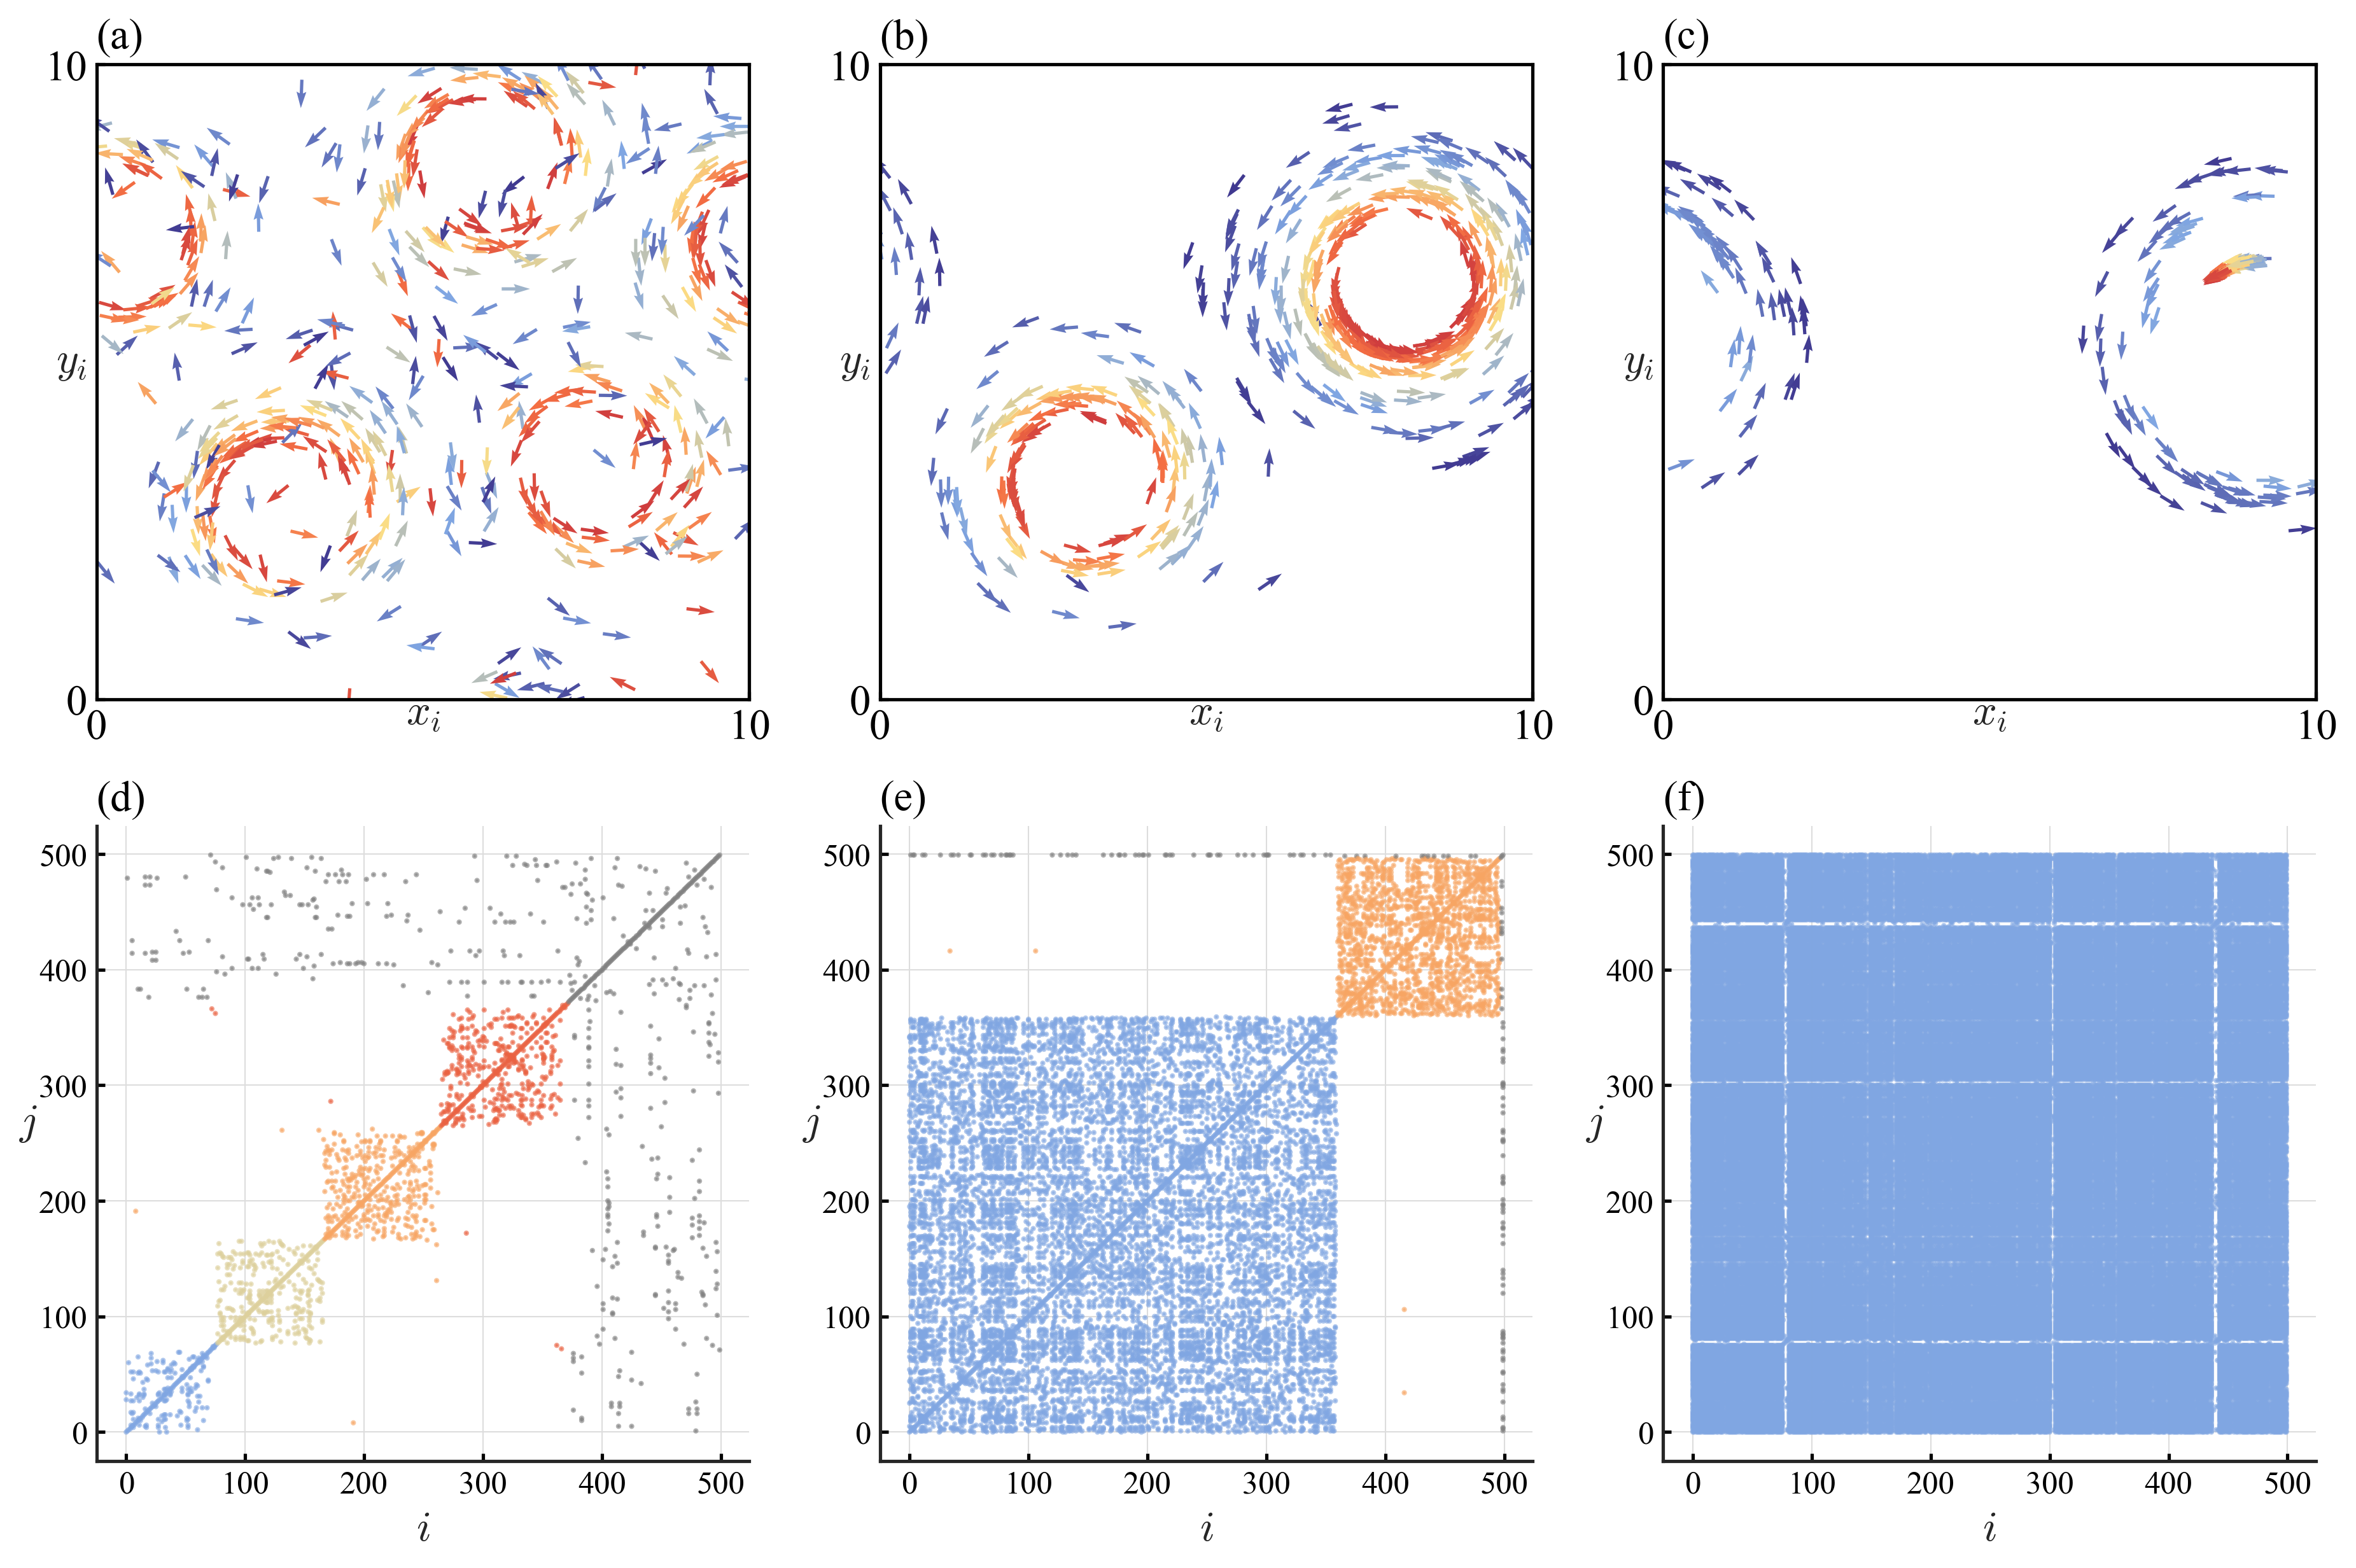
\includegraphics[width=\textwidth]{./figs/mono_CS_Aij.png}
%     \caption{
%         \label{fig:mono_CS_Aij}
%         Spatial clustering in the circling state of single-chiral swarmalators. 
%         Top row: snapshots of the spatial distribution of swarmalators. Bottom row: the adjacency matrix $A_{ij}$ of the network. 
%         \textbf{(a, d)}: $(\lambda, d_0)=(0.01, 0.35)$.
%         \textbf{(b, e)}: $(\lambda, d_0)=(0.01, 0.65)$.
%         \textbf{(c, f)}: $(\lambda, d_0)=(0.01, 1.05)$.
%         In \textbf{(d-f)}, only those elements $A_{ij}=1$ are plotted. The color of the matrix elements denotes different clusters, the gray elements represent the connections of the drifting swarmalators, and the white area represents the non-interacting region.
%     }
% \end{figure}

% Sorting the swarmalators within each cluster by their standardized spatial angles, which are defined as
% \begin{equation}
%     \arctan \left( \frac{y_i-\bar{Y}_i}{x_i-\bar{X}_i} \right)\;,
% \end{equation}
% where 
% \begin{equation}
%     \left[ \begin{array}{c}
%         \bar{Y}_i\\
%         \bar{X}_i\\
%     \end{array} \right] =\frac{1}{\left| C_k \right|}\sum_{i\in C_k}{\mathbf{c}_i}\;.
% \end{equation}

% \subsubsection{The Clustering State}
% Swarmalators in a cluster are phase synchronized and exhibit a spatial rotation at a unified synchronous frequency $\omega_s$. By summing over Eq.~(\ref{eq:additionalCouplingDotTheta}), one gets the aligned frequency as
% \begin{equation}
%     \label{eq:clusterState}
%     \begin{aligned}
%         \omega _s&=\frac{1}{N_c}\sum_{i=1}^{N_c}{\omega _i}+\frac{\lambda}{N_c}\sum_{i=1}^{N_c}{\sum_{j=1}^{N_c}{A_{ij}\sin \left( \theta _j-\theta _i \right)}}\\
%         &=\frac{1}{N_c}\sum_{i=1}^{N_c}{\omega _i}\;,\\
%     \end{aligned}
% \end{equation}
% where $N_c$ is the number of swarmalators in the cluster.

% \begin{figure}[H]
%     \centering
%     \includegraphics[width=0.7\textwidth]{./figs/Radii.pdf}
%     \caption{
%         \label{fig:radiusOmega} The real-time rotation radii of swarmalators in DS (blue, $d_0=0.1$, $\lambda=0.01:0.02$) and CS (orange, $d_0=0.1$, $\lambda=0.03:0.04$). The real-time rotation radii are close to $v/\omega_i$. 
%     }
% \end{figure}

% \begin{equation}
%     \begin{aligned}
%         X_i\left( t \right) &=x_i\left( t \right) -\frac{v}{\dot{\theta}_i\left( t \right)}\sin \theta _i\left( t \right)\;,\\
%         Y_i\left( t \right) &=y_i\left( t \right) +\frac{v}{\dot{\theta}_i\left( t \right)}\cos \theta _i\left( t \right)\;,\\
%     \end{aligned}
% \end{equation}

% \begin{figure}[H]
%     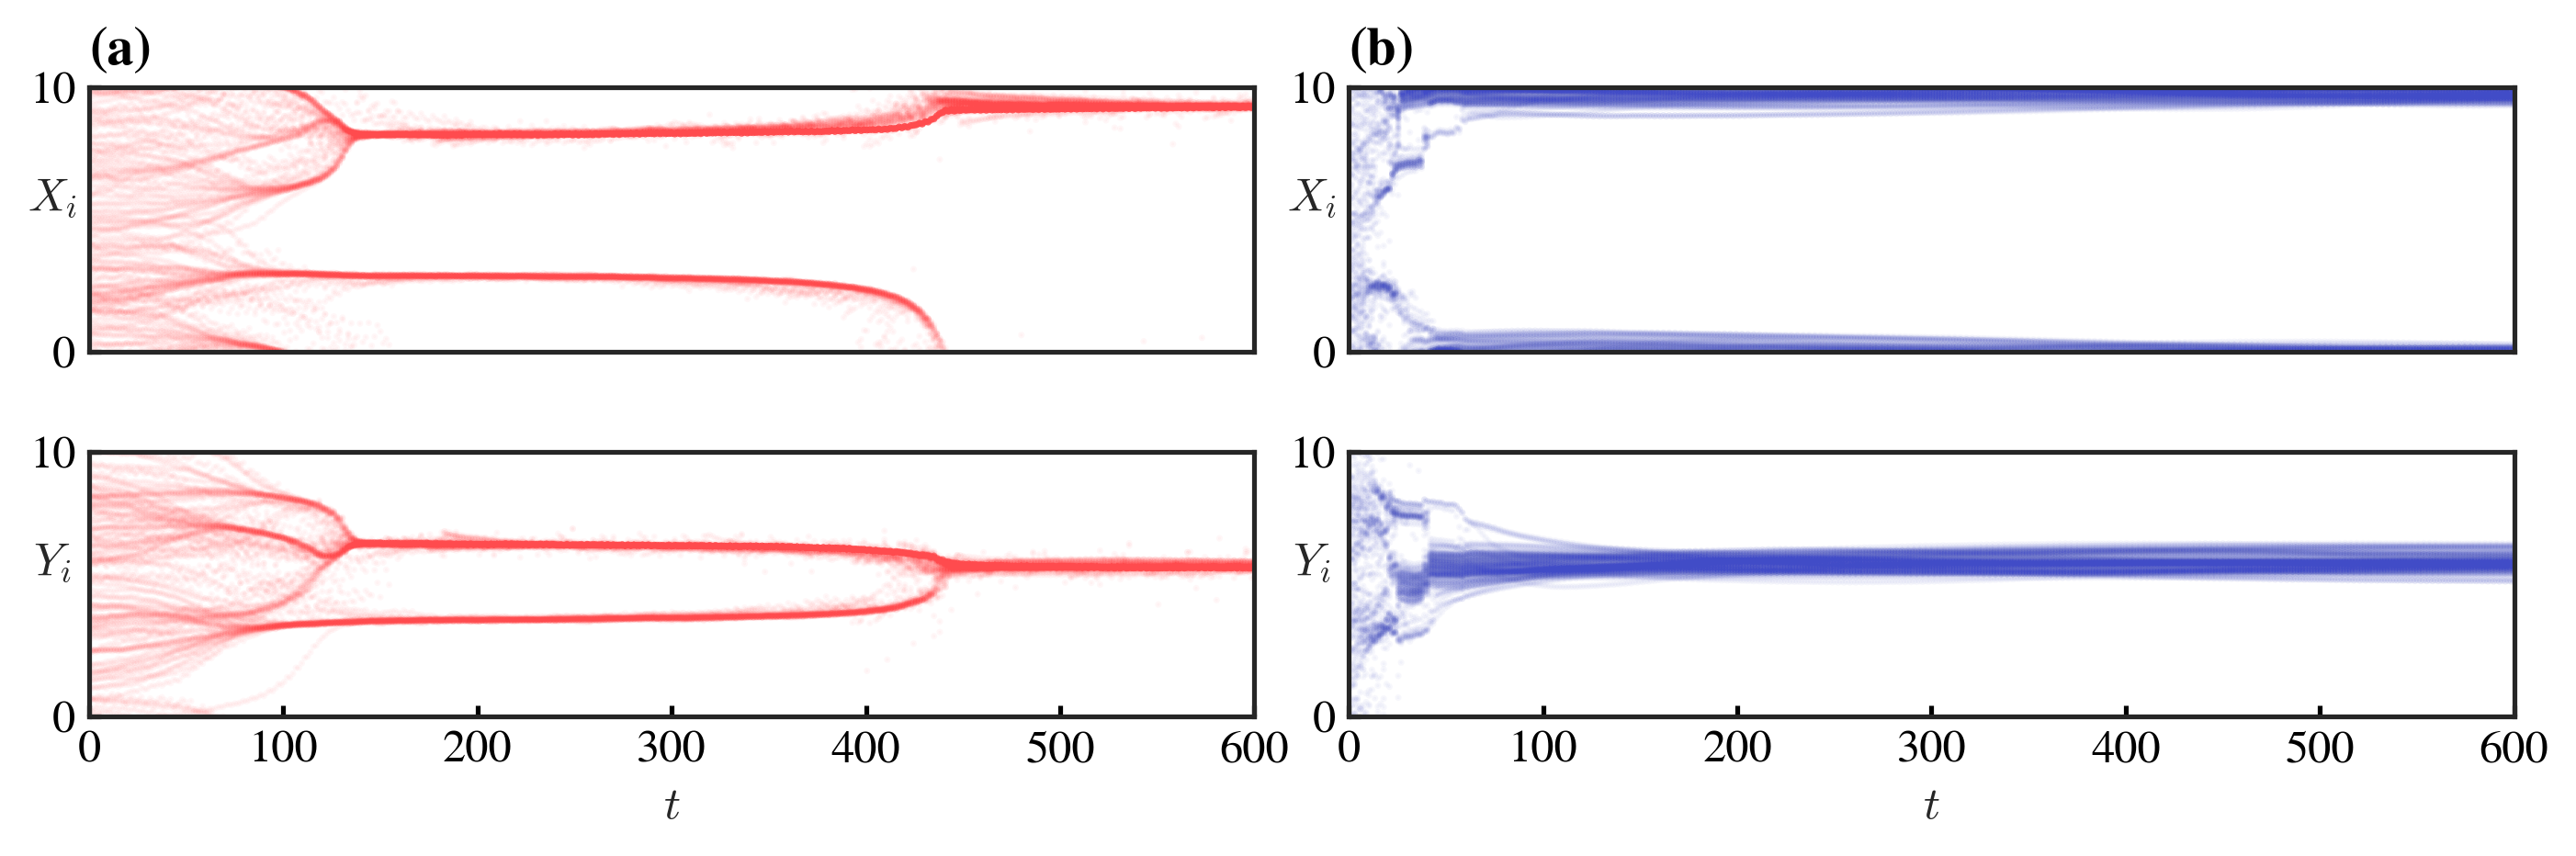
\includegraphics[width=\textwidth]{./figs/monoCentersPosition.png}
%     \caption{
%         \label{fig:monoCentersPosition} Scatter plot of the real-time centers of mono-chiral swarmalators.
%         \textbf{(a)}, centers position of CS ($\lambda=0.01$, $d_0=1$). 
%         \textbf{(b)}, centers position of CLS ($\lambda=0.045$, $d_0=1.05$). 
%         The color of the points denotes the corresponding natural frequency.
%     }
% \end{figure}

% \begin{figure}[H]
%     \centering
%     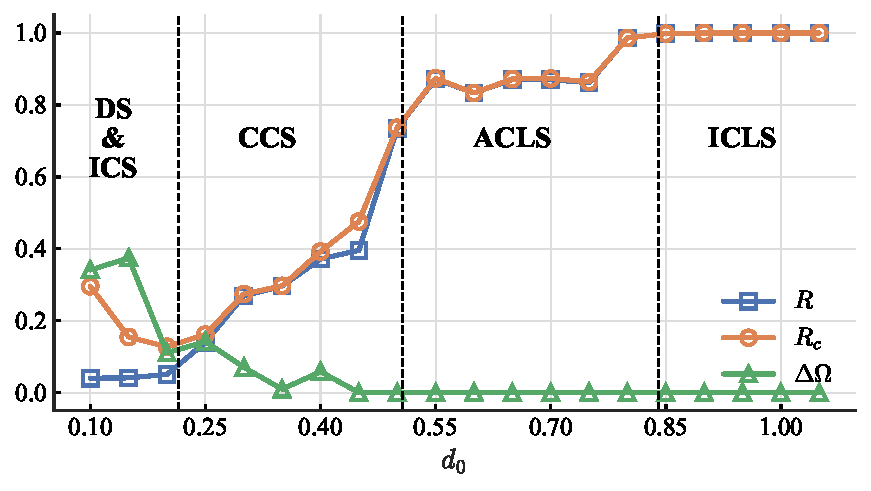
\includegraphics[width=0.7\textwidth]{./figs/monoOpPlot.pdf}
%     \caption{
%         \label{fig:monoOpPlot} Order parameters vary against $\lambda$ and $d_0$. 
%         \textbf{(a)}, $d_0=0.02$.
%         \textbf{(b)}, $\lambda=0.3$.
%         Blue, orange, green lines represent order parameters respectively for $R$, $R_c$ and $\Delta \Omega$.
%     }
% \end{figure}

% \subsection{Chiral Swarmalators}
% \begin{figure}[H]
%     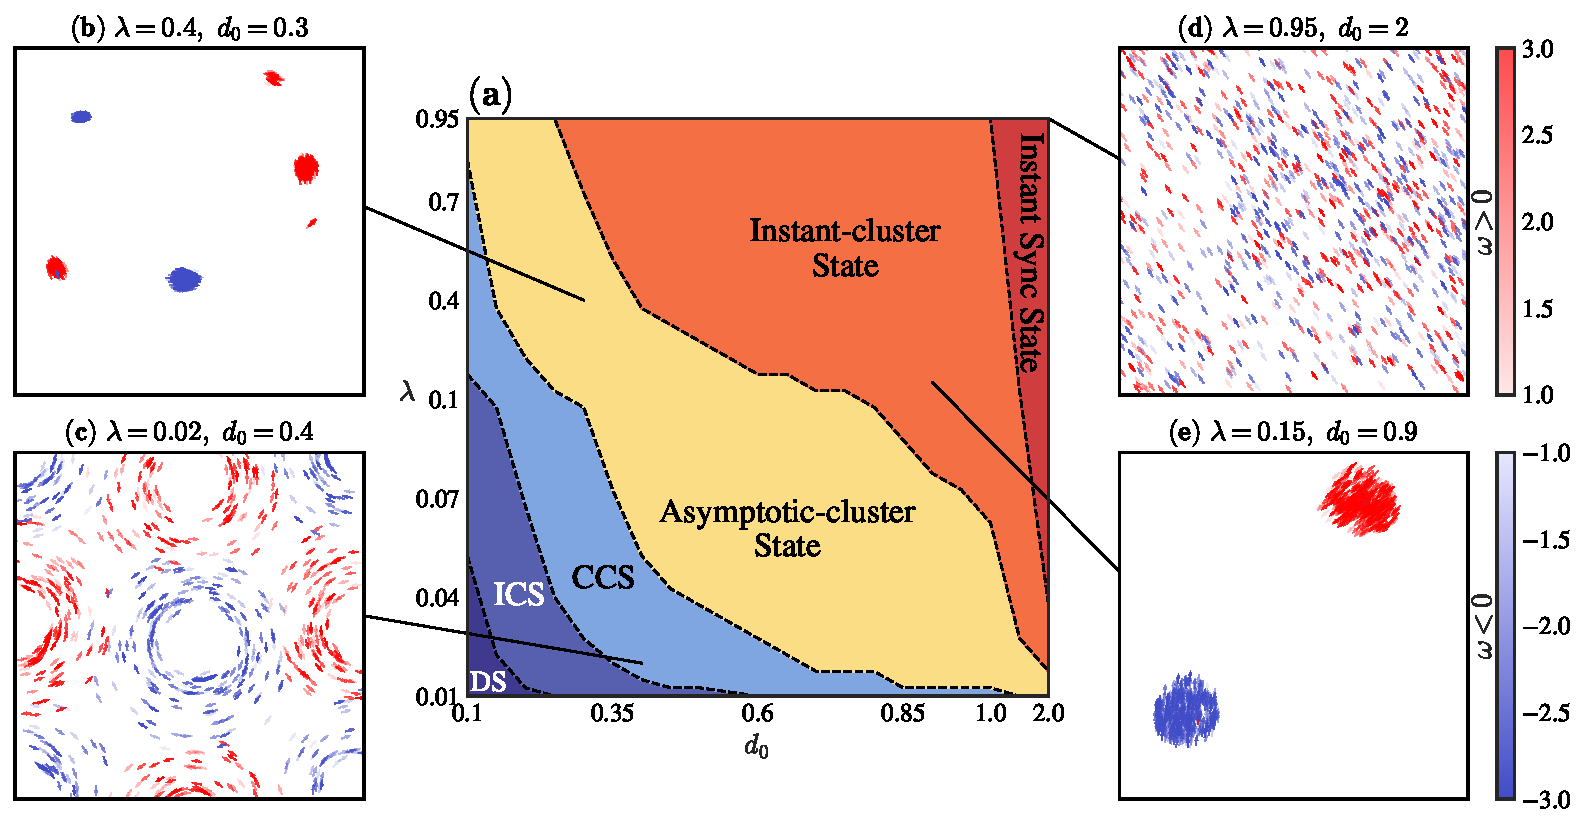
\includegraphics[width=\textwidth]{./figs/phaseDiagram.pdf}
%     \caption{
%         \label{fig:phaseDiagram} Phase diagram and snapshots of chiral swarmalators.
%         \textbf{(a)} Phase diagram in the $(d_0$-$\lambda)$ plane. The boundaries between states are analytical approximations given by Section~\ref{sec:phaseDiagrams}. 
%         For the sake of clarity, the scale of $\lambda$ and $d_0$ is non-uniform.
%         \textbf{(b)}, The snapshots of MCLS ($\lambda=0.4,\ d_0=0.3$). 
%         \textbf{(c)}, CS ($\lambda=0.02,\ d_0=0.4$).
%         \textbf{(d)}, ISS ($\lambda=0.95,\ d_0=2$).
%         \textbf{(e)}, DCLS ($\lambda=0.15,\ d_0=0.9$). 
%         Two types of chiral oscillators are represented by red ($\omega_i > 0$) and blue ($\omega_i < 0$) arrows, respectively. 
%     }
% \end{figure}

% \begin{figure}[H]
%     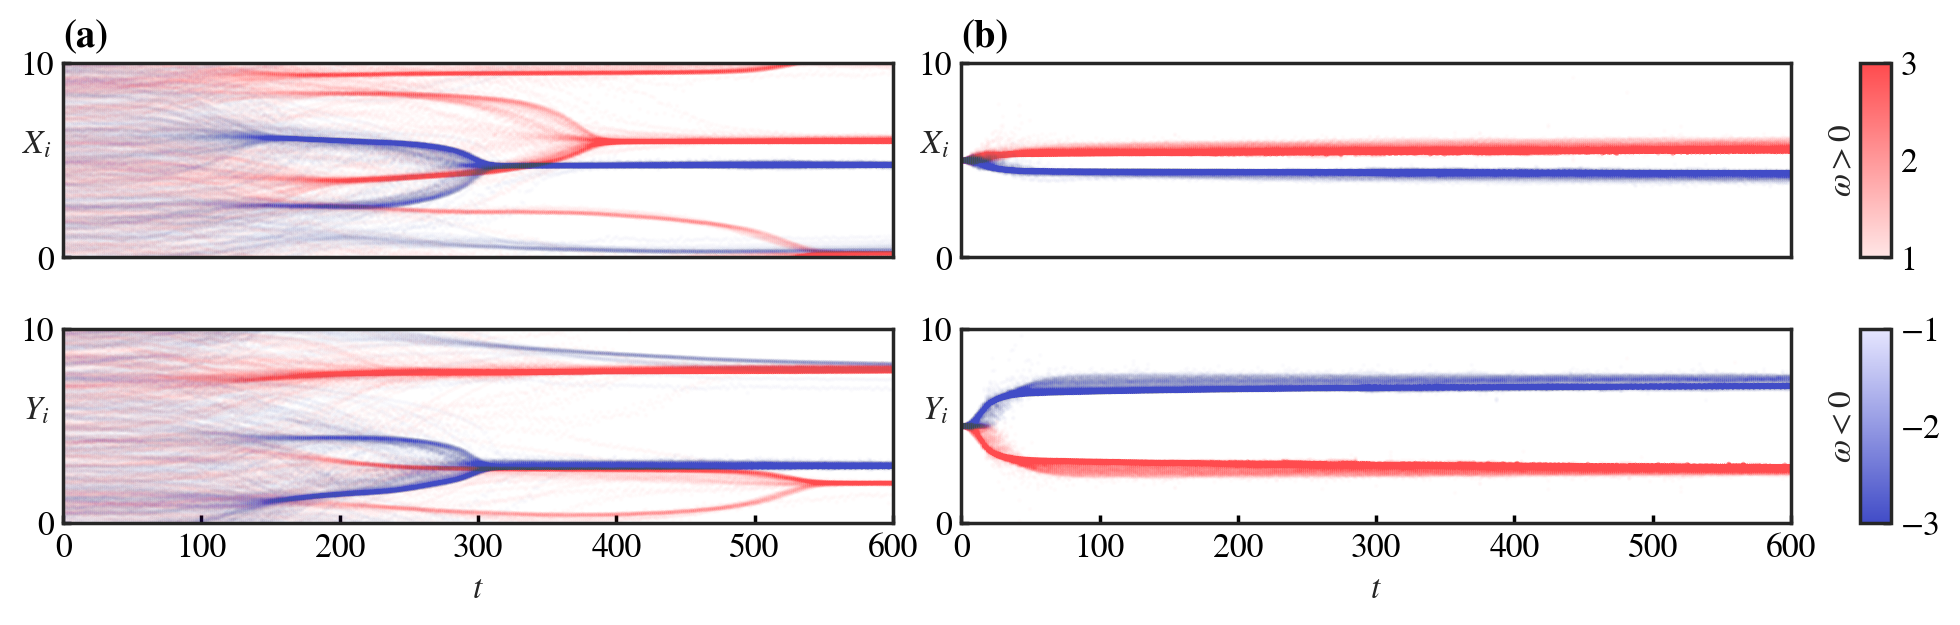
\includegraphics[width=\textwidth]{./figs/centersPosition.png}
%     \caption{
%         \label{fig:centersPosition} Scatter plot of the real-time centers of CS ($\lambda=0.02$, $d_0=0.4$).
%         \textbf{(a)}, behavior from random uniform initial condition. As time goes on, the centers of oscillators with the same chirality converge.
%         \textbf{(b)}, behavior from clustered initial condition. The centers of swarmalators are already clustered at a concentric ring.
%         The color of the points denotes the corresponding natural frequency.
%     }
% \end{figure}

% \begin{figure}[H]
%     \centering
%     \includegraphics[width=\textwidth]{./figs/Aij.png}
%     \caption{
%         \label{fig:Aij} The adjacency matrix $A_{ij}$ of chiral swarmalators. 
%         \textbf{(a)}, $A_{ij}$ of CS ($\lambda=0.02$, $d_0=0.4$).
%         \textbf{(b)}, $A_{ij}$ of CLS ($\lambda=0.15$, $d_0=0.9$).
%         The color of the point denotes the corresponding cluster index. No color means the $i$th swarmalator is not connected to $j$th swarmalator.
%     }
% \end{figure}

% \newpage
% \section{Mechanism of Condensation and Separation Dynamics}

% \begin{figure}[H]
%     \centering
%     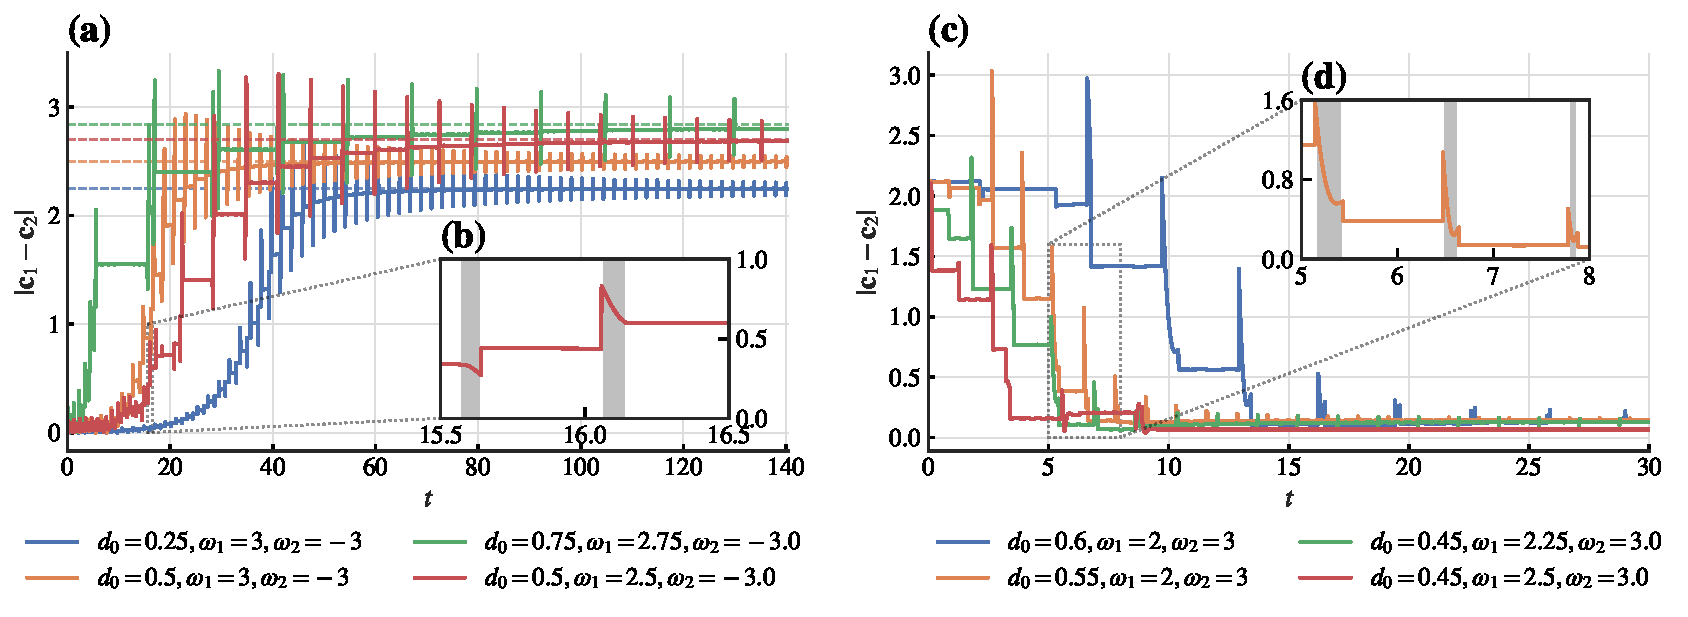
\includegraphics[width=0.7\textwidth]{./figs/2OsCenterDistance.pdf}
%     \caption{
%         \label{fig:2OsCenterDistance} The distance between the centers of two swarmalators ($\lambda=1$). 
%         \textbf{(a)}, The distance between the centers of two chiral swarmalators. The dashed line is the theoretical maximum distance.
%         \textbf{(b)}, The distance between the centers of two mono-chiral swarmalators.
%     }
% \end{figure}

% \newpage
% \section{Phase Diagrams and Critical Thresholds\label{sec:phaseDiagrams}}

% \newpage
% \begin{figure}[H]
%     \centering
%     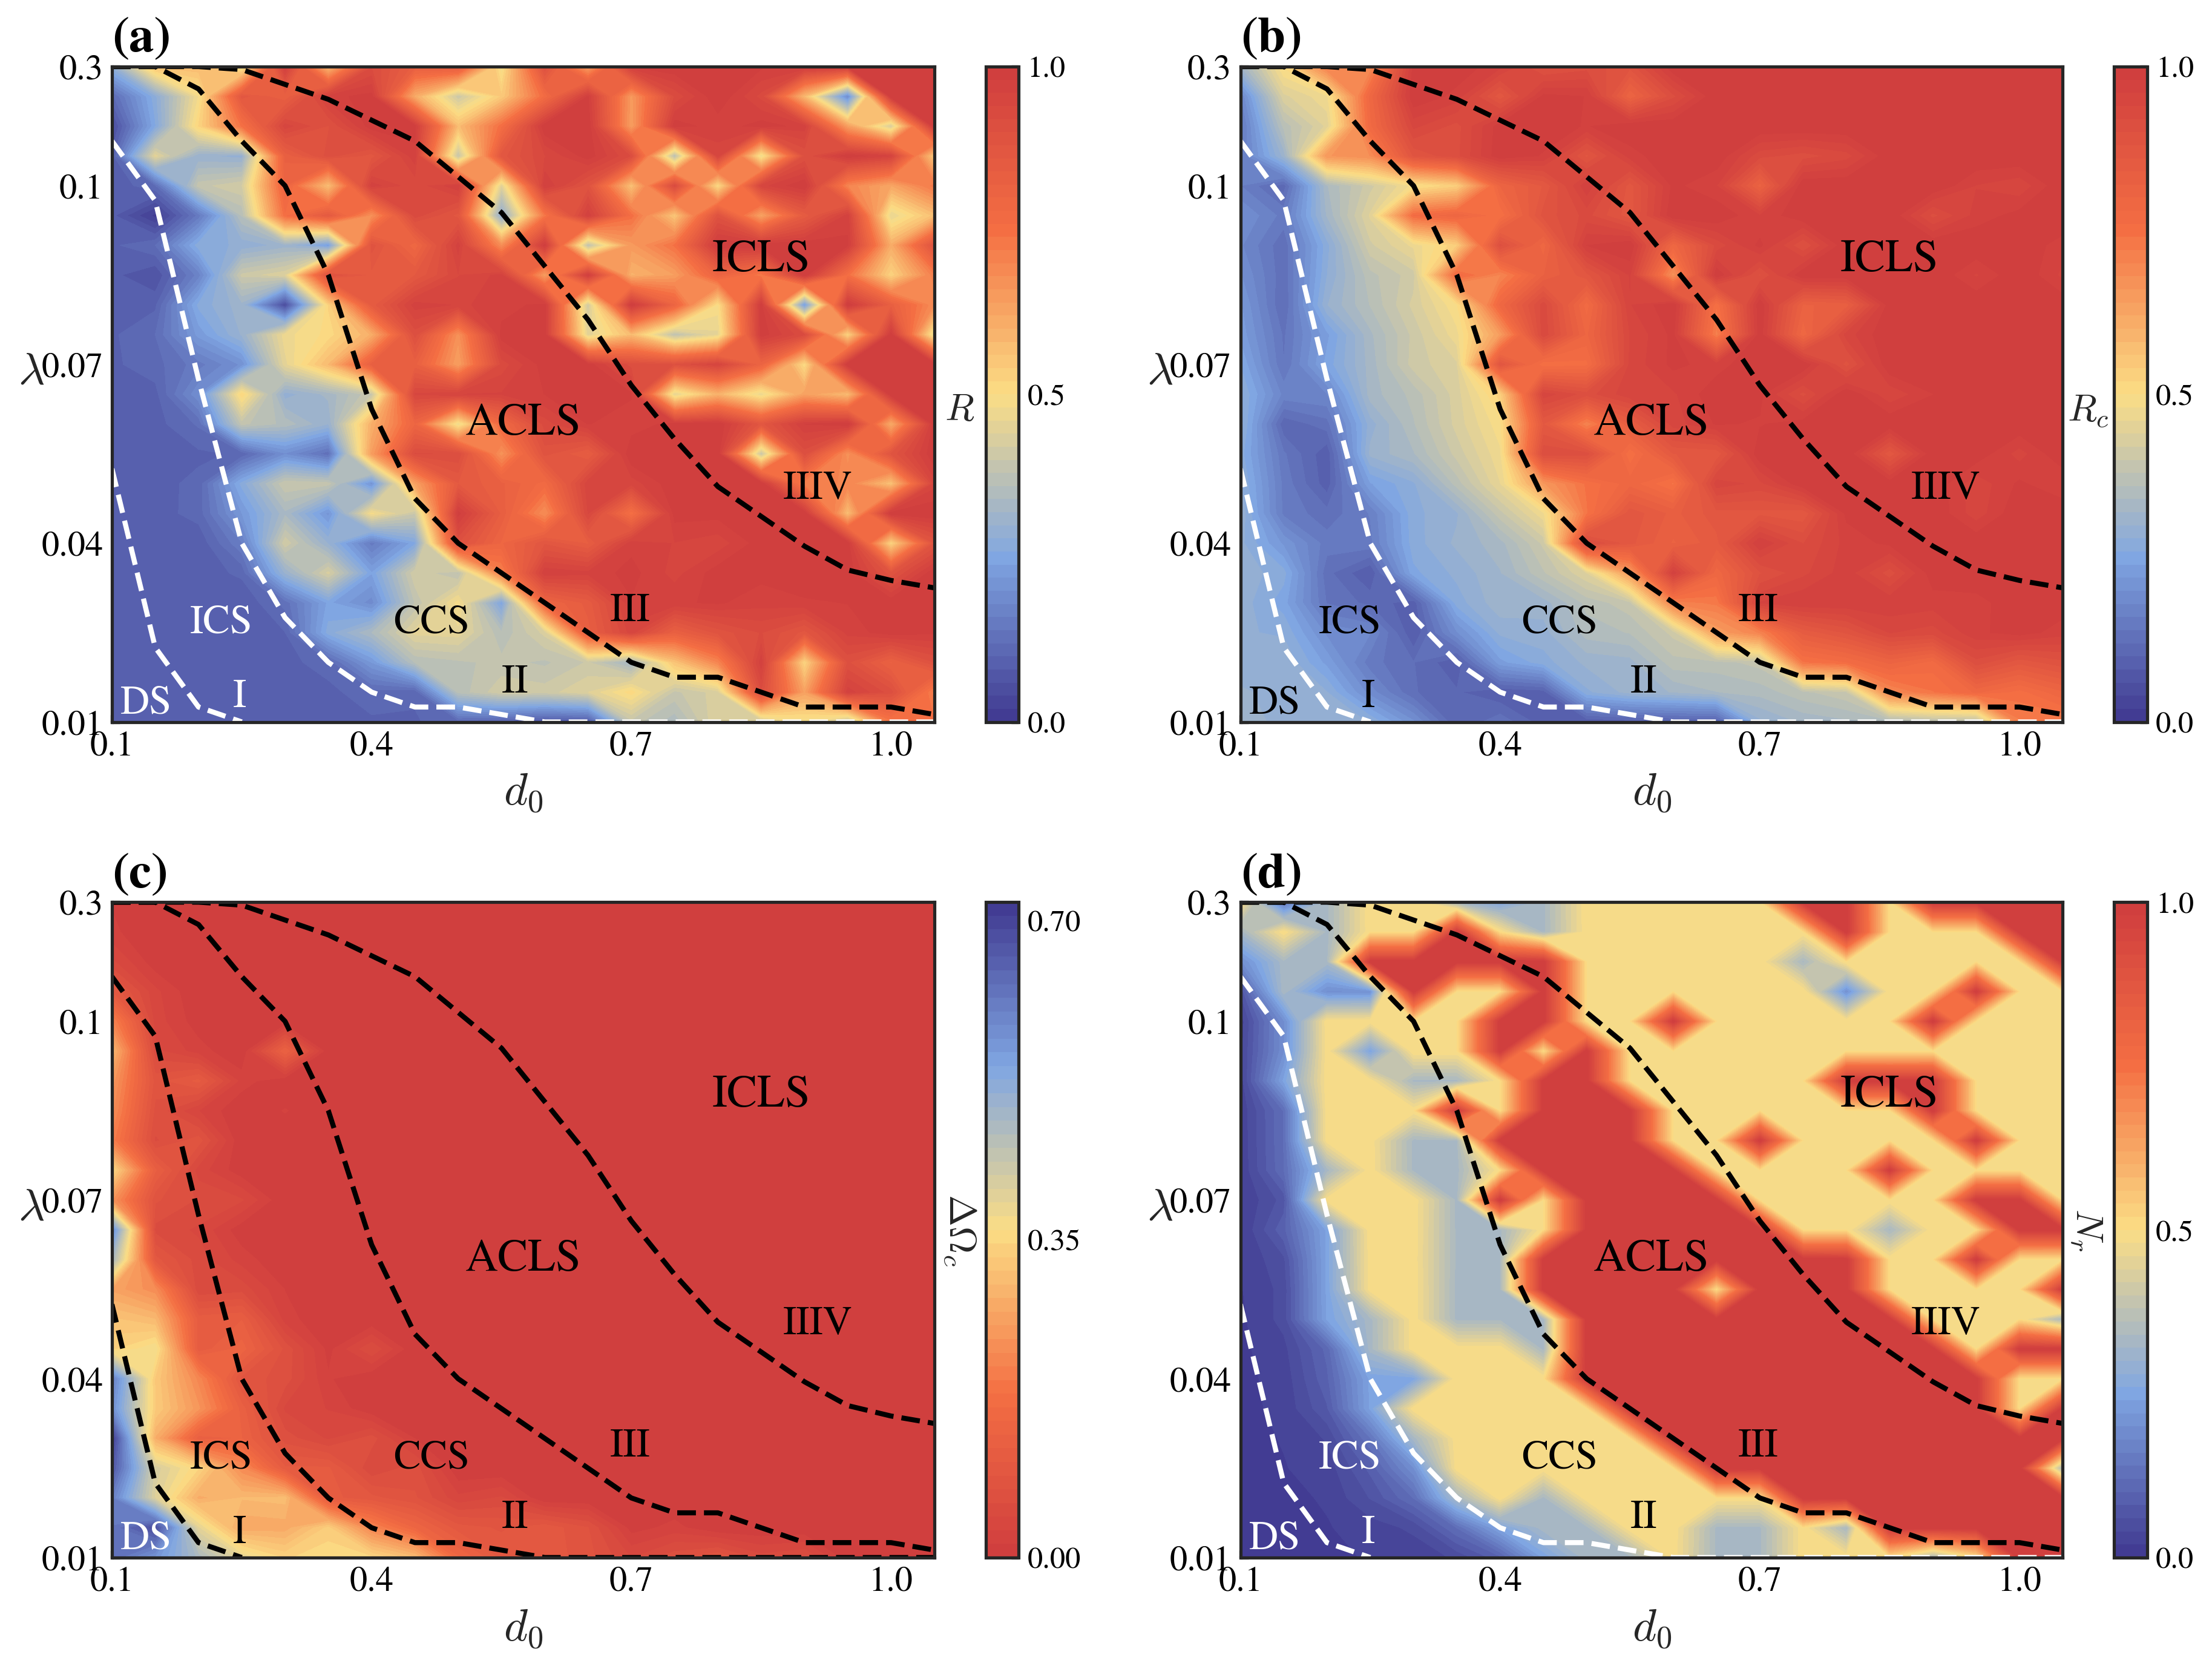
\includegraphics[width=0.75\textwidth]{./figs/monoOrderParam.png}
%     \caption{
%         \label{fig:monoOrderParam} Heatmaps for different order parameters of single-chiral swarmalators across the ($\lambda$, $d_0$) plane and the critical lines of the transitions between states.
%         \textbf{(a)-(d)} correspond to the order parameters $R$, $R_c$, $\Delta \Omega_c$ and $N_r$, respectively.
%         Different colors describe the amplitudes of different order parameters.
%     }
% \end{figure}

% \begin{figure}[H]
%     \centering
%     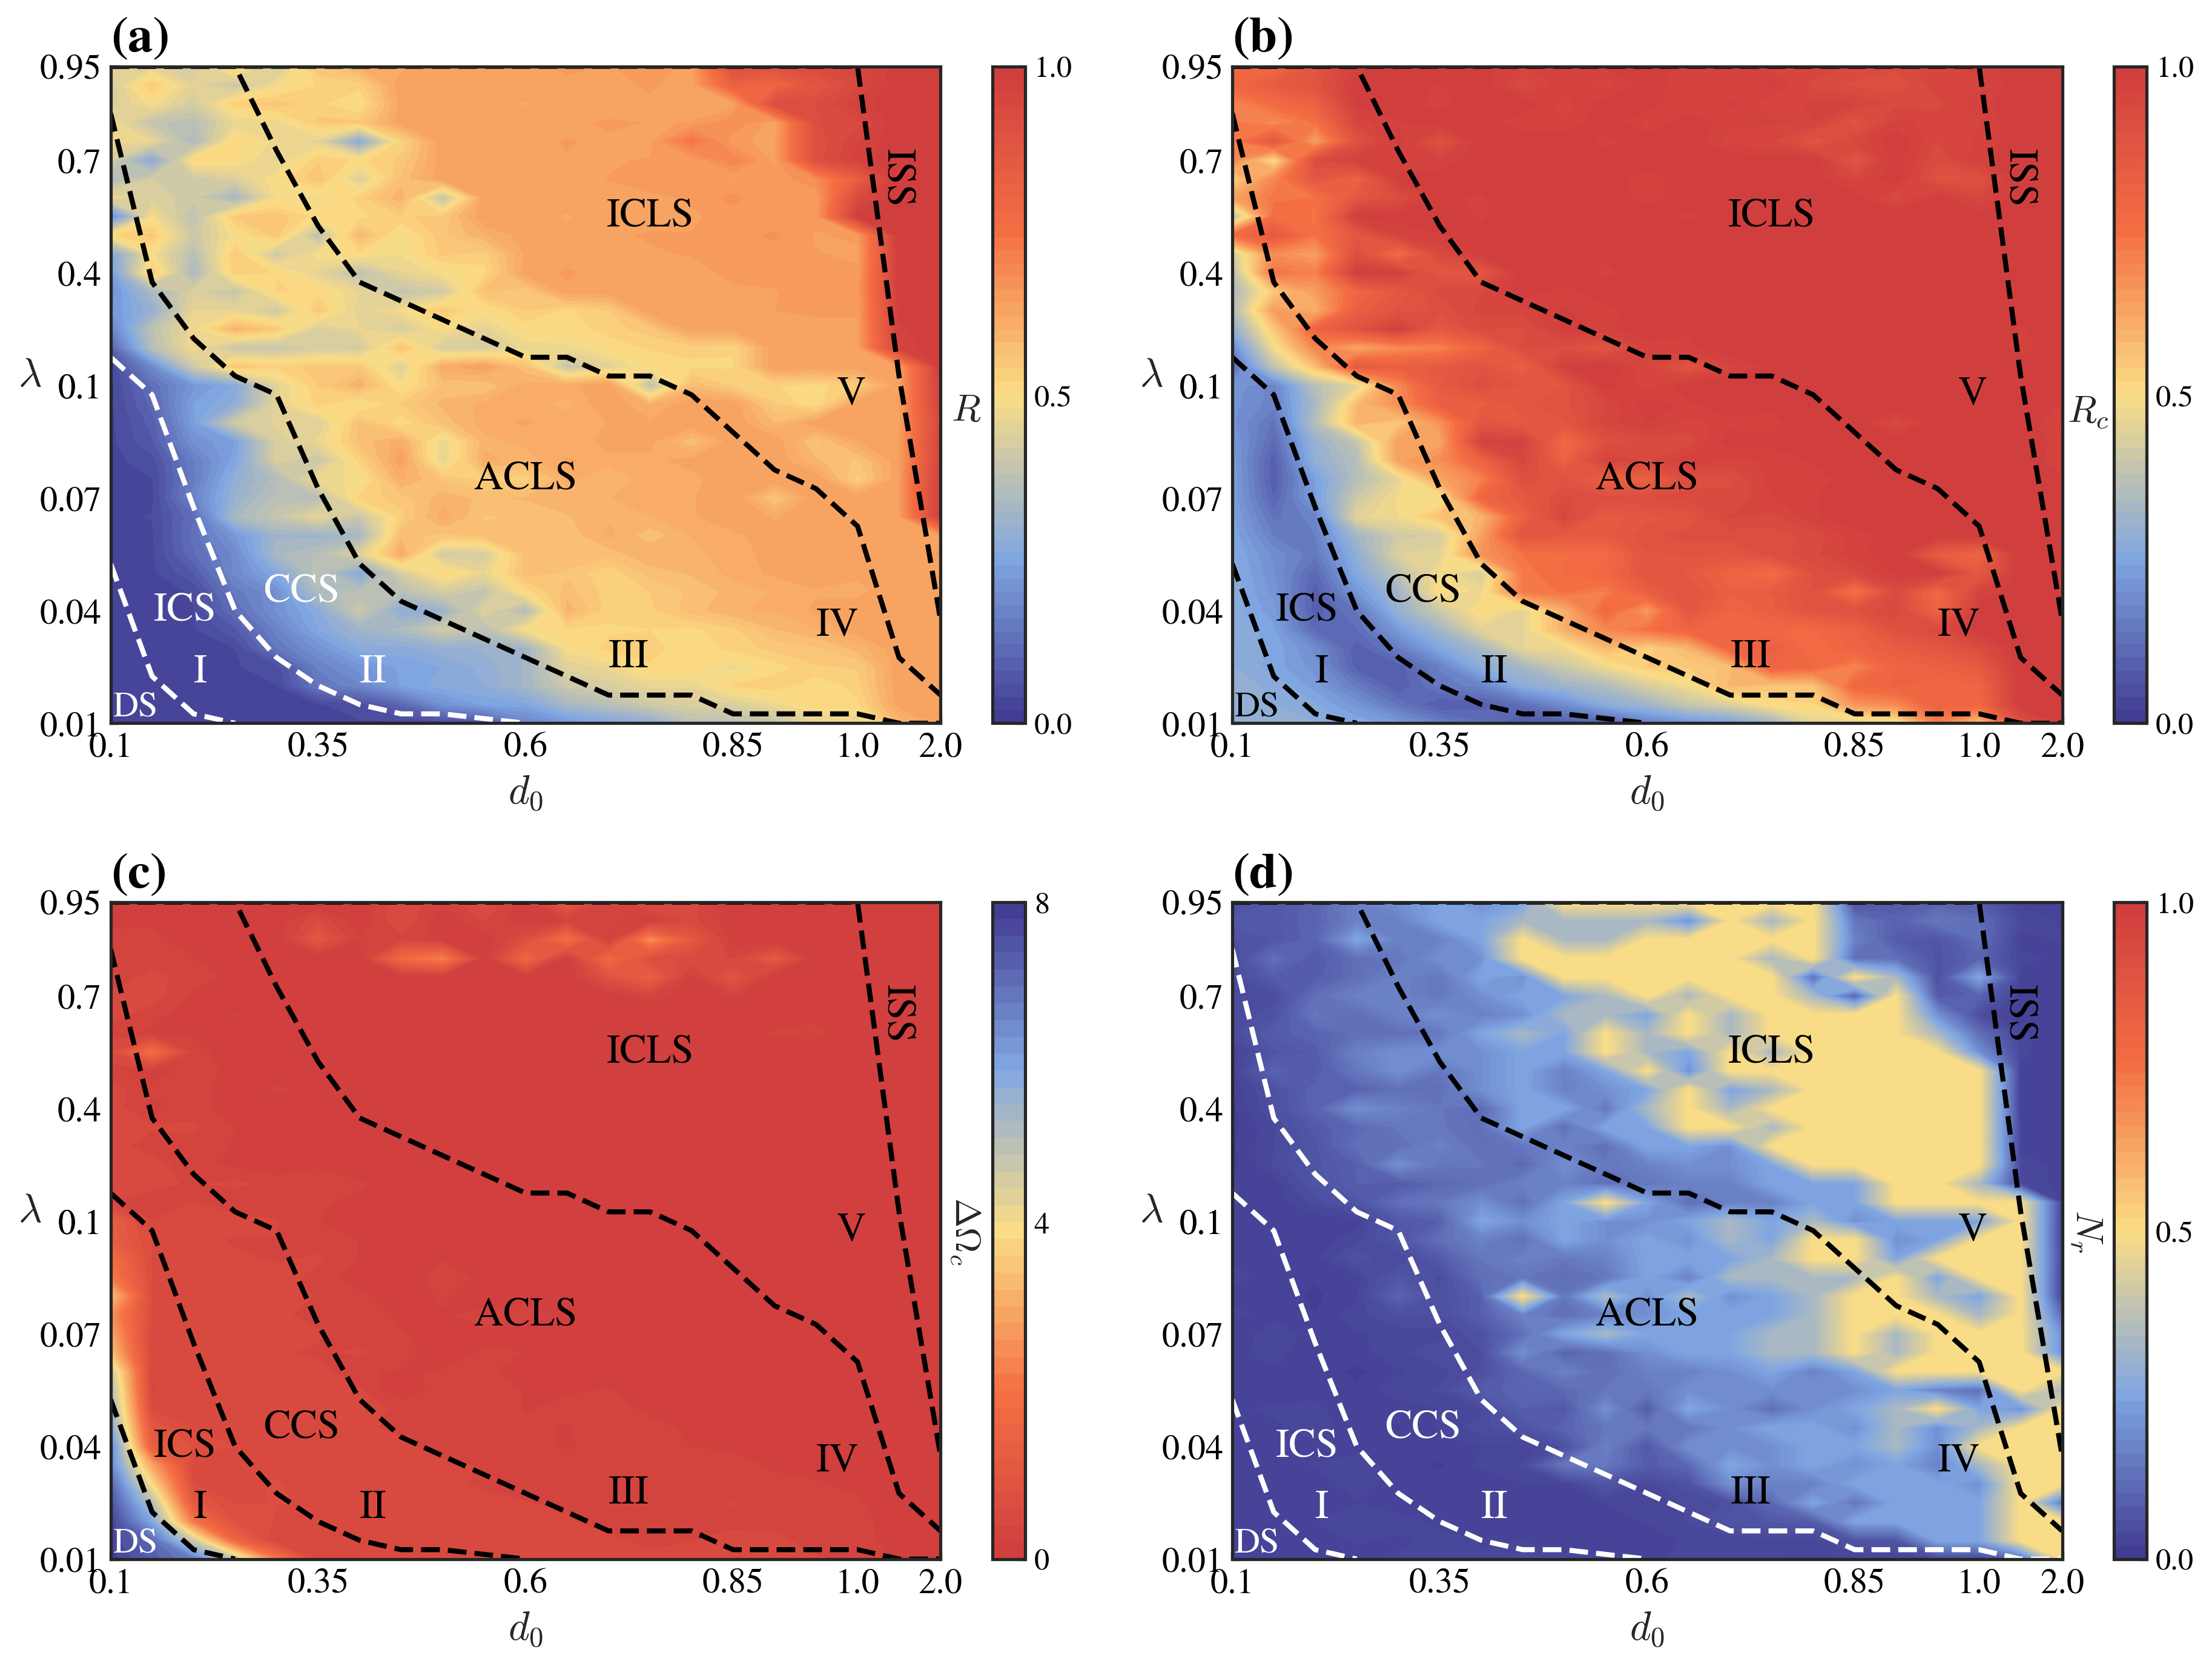
\includegraphics[width=0.75\textwidth]{./figs/orderParam.png}
%     \caption{
%         \label{fig:orderParam} Heatmaps for different order parameters of double-chiral swarmalators across the ($\lambda$, $d_0$) plane and the critical lines of the transitions between states.
%         \textbf{(a)-(d)} correspond to the order parameters $R$, $R_c$, $\Delta \Omega_c$ and $N_r$, respectively.
%         Different colors describe the amplitudes of various order parameters.
%     }
% \end{figure}

% \begin{figure}[H]
%     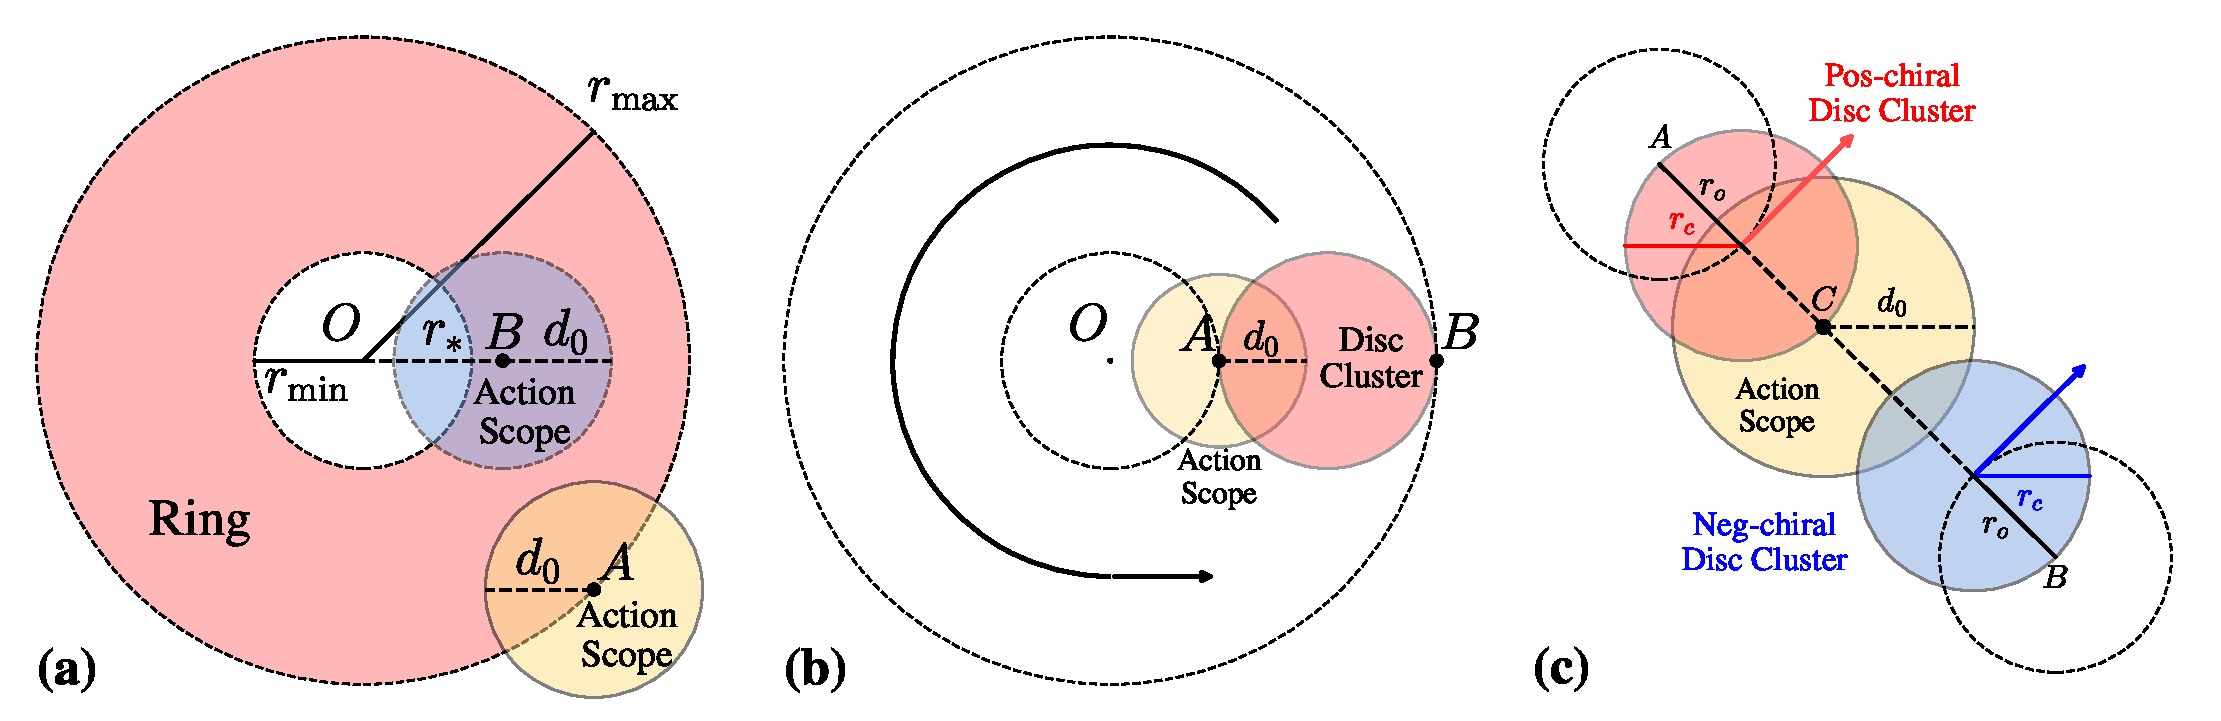
\includegraphics[width=\textwidth]{./figs/analyticalEps.pdf}
%     \caption{
%         \label{fig:analyticalEps}
%         The schematic plot of the analytical approximations.
%         \textbf{(a)}, The $1$st oscillator is at point $A$ which is on the outer edge of the ring, and the overlapping area of the yellow circle (action scope) and the red ring is $S_1\left( d_0 \right)$.
%         \textbf{(b)}, The $1$st oscillator is at point $A$ which is on the inner edge of the ring, and the overlapping area of the yellow circle (action scope) and the red ring is $S_2\left( d_0 \right)$.
%         \textbf{(c)}, The $1$st oscillator is at point $C$ which is on the edge of red circle, and the overlapping area of the yellow circle (action scope) and the blue circle is $S_3\left( d_0 \right)$.
%     }
% \end{figure}

% \begin{equation}
%     \begin{cases}
%         \lambda _{c1}=\frac{\pi \left( r_{\max}^{2}-r_{\min}^{2} \right) \left( \omega _{\max}-\omega _{\min} \right)}{N_{c}^{2}\left( d_{0}^{2}\frac{\alpha}{2}+r_{\max}^{2}\frac{\beta}{2}-r_{\max}d_0\sin \frac{\alpha}{2} \right)}\\
%         \beta =2\mathrm{arc}\cos \left( 1-\frac{d_{0}^{2}}{2r_{\max}^{2}} \right)\\
%         \alpha =\pi -\frac{\beta}{2}\\
%     \end{cases}\;.
% \end{equation}

% \begin{equation}
%     \begin{cases}
%         \lambda _{c2}=\frac{\pi r_{s}^{2}\left( \omega _{\max}-\omega _{\min} \right)}{N_S\left( d_{0}^{2}\frac{\alpha}{2}+r_{s}^{2}\frac{\beta}{2}-r_sd_0\sin \frac{\alpha}{2} \right)}\\
%         \beta =2\mathrm{arc}\cos \left( 1-\frac{d_{0}^{2}}{2r_{s}^{2}} \right)\\
%         \alpha =\pi -\frac{\beta}{2}\\
%         r_s=\frac{r_{\max}-r_{\min}}{2}\\
%     \end{cases}\;.
% \end{equation}

% \begin{equation}
%     \lambda _{c3}=\frac{L^2\left( \omega _{\max}-\omega _{\min} \right)}{N\pi d_{0}^{2}}\;.
% \end{equation}

% \begin{equation}
%     \begin{cases}
%         \lambda _{c4}=\frac{2\pi r_{s}^{2}\omega _{\max}}{N_c\left( \frac{\alpha}{2}r_{s}^{2}+\frac{\beta}{2}d_{0}^{2}-d_0r_d\sin \frac{\beta}{2} \right)}\\
%         r_d=\frac{L}{\sqrt{2}}-r_s-2r_c\\
%         \beta =2\mathrm{arc}\cos \frac{d_{0}^{2}+r_{d}^{2}-r_{s}^{2}}{2d_0r_d}\\
%         \alpha =2\mathrm{arc}\cos \frac{r_{s}^{2}+r_{d}^{2}-d_{0}^{2}}{2r_sr_d}\\
%     \end{cases}\;.
% \end{equation}

% \newpage
% \section{Self-consistency Equation}

% Inspired by global order parameter $R$, one can define the local order parameter $R_i$:
% \begin{equation}
%     \label{eq:localOrderParameter}
%     R_{c}^{i}\mathrm{e}^{\mathrm{i}\psi _{c}^{i}}=\frac{1}{\left| C_i \right|}\sum_{j\in C_i}{\mathrm{e}^{\mathrm{i}\theta _j}}\;,
% \end{equation}
% where $C_i=\left\{ j\mid \Delta r_{ij}\le d_0 \right\}$. If the swarmalators in set $C_i$ are the initial to entry the coherent state, and other swarmalators are still in the incoherent state, then the $R_i$ will bifurcate from zero simultaneously with $R$ and $R_c$. Then the Eq.~\eqref{eq:swarmalatorDotTheta} can be rewritten as
% \begin{equation}
%     \label{eq:localDotTheta}
%     \dot{\theta}_i=\omega _i+\frac{K}{N} \sum_{j\in C_i}{\sin \left( \theta _j-\theta _i \right)}\;.
% \end{equation}
% By introducing $\Sigma _2\left( d_0 \right) =\sum\nolimits_{j\in C_i}^{}{A_{ij}}=\left|C_i\right|$, Eq.~\eqref{eq:localOrderParameter} becomes 
% \begin{equation}
%     \frac{K\Sigma _2R_{c}^{i}}{N} \sin \left( \psi _{c}^{i}-\theta _i \right) =\frac{K}{N} \sum_{j\in C_k}{\sin \left( \theta _j-\theta _i \right)}
% ;.
% \end{equation}
% Then by introducing $\varphi _i=\theta _i-\bar{\omega}t=\theta_i-\psi _{c}^{i}$, where $\bar{\omega}=\sum_{j\in C_i}{\omega _j}/\left| C_i \right|$ is synchronous frequency of the swarmalators in $C_i$ given by Eq.~(\ref{eq:clusterState}), Eq.~(\ref{eq:localDotTheta}) can be recast as
% \begin{equation}
%     \label{eq:dotphi}
%     \dot{\varphi}_i=\dot{\theta}_i-\bar{\omega}-\frac{K\Sigma _2R_{c}^{i}}{N} \sin \varphi _i\;.
% \end{equation}

% When $N\rightarrow \infty$, the mean field can be expressed by the distribution function as
% \begin{equation}
%     R_{c}^{i}\mathrm{e}^{\mathrm{i}\psi _{c}^{i}}=\mathrm{e}^{\mathrm{i}\bar{\omega}t}\int_0^{2\pi}{\int_{-\infty}^{\infty}{\mathrm{e}^{\mathrm{i}\varphi}}}P(\varphi ,\omega ,t)g(\omega )\mathrm{d}\omega \mathrm{d}\varphi\;.
% \end{equation}

% \newpage
% \section{Appendix}

% \begin{figure}[H]
%     \centering
%     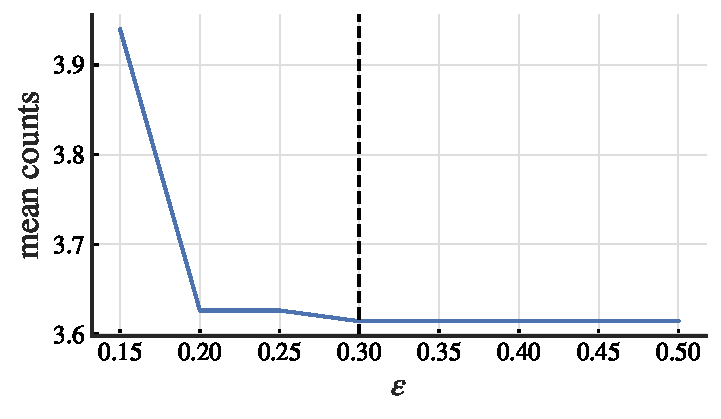
\includegraphics[width=0.7\textwidth]{./figs/DBSCANparam.pdf}
%     \caption{
%         \label{fig:DBSCANparam} The minimum counts of clusters with $m=0$ and different $\varepsilon$. The number of clusters is calculated by DBSCAN algorithm. The mean counts converges at $\varepsilon=0.3$.
%     }
% \end{figure}

% \begin{figure}[H]
%     \centering
%     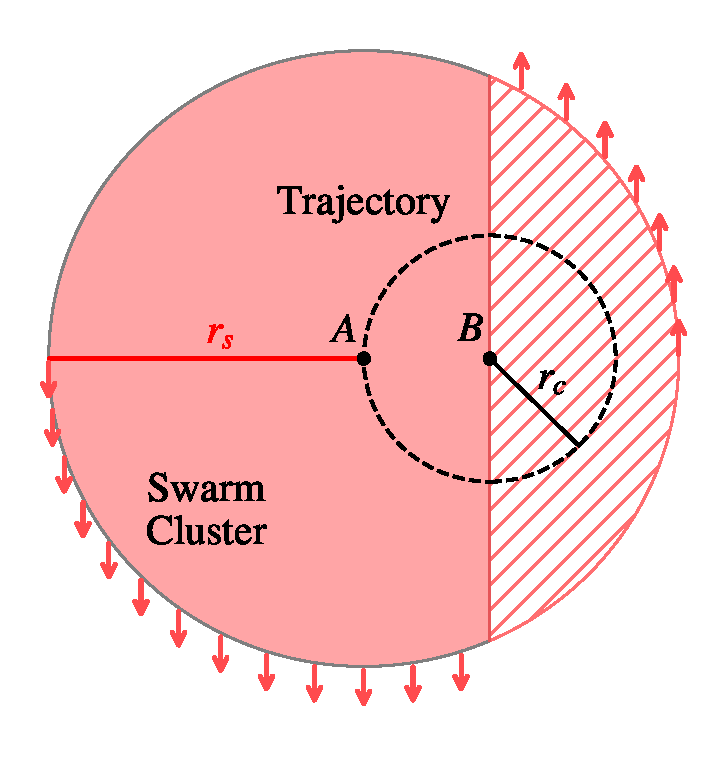
\includegraphics[width=0.6\textwidth]{./figs/rsProofEps.pdf}
%     \caption{
%         \label{fig:rsProofEps} The schematic plot of $r_s>r_c$.
%     }
% \end{figure}

\bibliography{ref}

\end{document}